\documentclass{unicam_thesis}
\usepackage[utf8]{inputenc}
\usepackage{listings}
%%%%%%%%%%%%%%%%%%%%%%%%%%%%
% FRONTESPIZIO
%%%%%%%%%%%%%%%%%%%%%%%%%%%%

\title{Editor di oggetti 3D per e-commerce configurabile e in realt\`a aumentata: \\ il backend di “Customyzx”}

\university{Universit\`a degli Studi di Camerino}%
\school{Scienze e Tecnologie}%
\course{Laurea in Informatica (Classe L-31)}%


\author{Paolo Andreassi}%
\advisor{Dott. Francesco De Angelis}%
\coadvisor2{Dott. Antonio dell'Ava}%
\academicyear{2017/2018}%
\matricola{090629}%

%%%%%%%%%%%%%%%%%%%%%%%%%%%%
% FINE FRONTESPIZIO
%%%%%%%%%%%%%%%%%%%%%%%%%%%%


\theoremstyle{definition} \newtheorem{esempio}{Esempio}[chapter]
\theoremstyle{definition}
\newtheorem{definizione}{Definizione}[chapter] \theoremstyle{plain}
\newtheorem{teorema}{Teorema}[chapter]

\graphicspath{{Screenshot/},{Immagini/},{Source/}}
\bibliography{biblio.bib}
\begin{document}

\maketitle

\tableofcontents
\lstlistoflistings
\listoffigures

\chapter{Introduzione}
\label{chap:intro}
La qui presente tesi rappresenta la terza ed ultima parte dello stage++\footnote{Lo stage++ è un progetto unico che comprende l'insieme di tre moduli: stage, project work e tesi.}, che è stato realizzato in collaborazione con il Prof. Francesco De Angelis, e-xtrategy s.r.l. e con il collega Filippo Corona.
Durante lo stage ci è stato chiesto di progettare e realizzare un’applicazione per la visualizzazione e l'editing di modelli
3D da impiegare in ambito e-commerce.
Il prodotto che ne è risultato ha preso il nome di "CustoMyzx".

Per poter raggiungere i numerosi obettivi che questo progetto richiedeva, io e Filippo ci siamo divisi il carico di lavoro in maniera il più possibile equa: una metà del progetto si è focalizzata sul front end, e quindi sull’interfaccia mirata all’utente, l’altra invece sul back end, estraneo a quest’ultimo.
Nella prima fase della progettazione, i due semi-progetti sono stati nominati rispettivamente “unicam-product-viewer” e “unicam-product-editor” ai fini di una distinzione tra questi.
Io mi sono occupato della parte back end, e quindi di "unicam-product-editor", mentre Filippo, in modo complementare, ha sviluppato la parte front end e il relativo sotto-progetto:"unicam-product-viewer".

Quindi il progetto è composto dalle seguenti parti:
\begin{enumerate}
	\item Il back end
	\item Una web app come interfaccia per il back end
	\item Il front end
	\item Il configuratore 3D e in realtà aumentata sviluppato tramite web app
\end{enumerate}
Tutte le parti di CustoMyzx sono state scritte in Javascript ad eccezione di uno script esterno realizzato in Python.

Questa tesi tratterà nella fattispecie i primi due punti: la realizzazione dell'applicazione web mediante l'utilizzo del MEAN Stack\index{MEAN} piuttosto che il tradizionale LAMP Stack\footnote{Acronimo (Linux, Apache, MySQL, PHP) che indica una piattaforma software per lo sviluppo di applicazioni web}, e l'uso del modello architetturale nelle web app chiamato "Long Polling".

Il codice completo del progetto è disponibile nei due repository
\begin{enumerate}
	\item \url{www.github.com/e-xtrategy/unicam-product-editor}
	\item \url{www.github.com/e-xtrategy/unicam-product-viewer}
\end{enumerate} 

\section{Progettazione}
La fase di progettazione si è sviluppata secondo il metodo extrategy: l'azienda basa lo sviluppo di software sulle metodologie agili, più adatte ad ambienti dinamici come lo è il web, come ad esempio la formazione di team di sviluppo piccoli, cross-funzionali e auto-organizzati, 
lo sviluppo iterativo e incrementale, la pianificazione adattiva, e il coinvolgimento diretto e continuo del cliente nel processo di sviluppo.

In particolare, abbiamo utilizzato una via di mezzo tra Scrum e Kanban.

L'utilizzo del framework Scrum\cite{scrum}\index{Scrum} consiste nel passaggio attraverso una serie di iterazioni a intervalli di tempo regolari, dette sprint\index{Sprint}, che consentono di consegnare il progetto passo dopo passo al cliente e con cadenza costante. Attraverso la giusta frequenza adottata per gli sprint, si è capaci di fare delle stime più corrette, e inoltre si possono ricevere feedback in tempo reale sul lavoro svolto.
Ogni sprint si divide in quattro fasi:
\begin{enumerate}
	\item \textbf{Pianificazione}: incontro iniziale in cui si definisce cosa fare con lo sprint corrente.
	\item \textbf{Scrum giornaliero}: mini incontro giornaliero della durata di una decina di minuti per sincronizzare il team. 
	\item \textbf{Demo}: incontro per illustrare il lavoro svolto dal team.
	\item \textbf{Retrospettiva}: una revisione di ciò che è stato fatto, esponendo anche i possibili miglioramenti attuabili.
\end{enumerate} 

Il Kanban\cite{kanban}\index{kanban} serve per tenere d'occhio l'avanzamento dei lavori durante gli sprint; la kanban board dunque non è altro che una lavagna atta a visualizzare e ottimizzare il flusso di lavoro del team. Un classico kanban può essere dato da una lavagna o da un' intera parete (es. e-xtrategy), ma per il nostro sviluppo software abbiamo utilizzato una board virtuale, in cui abbiamo riscontrato aspetti positivi quali tracciabilità, facilità di collaborazione, accessibilità delocalizzata.

Le funzioni di una kanban sono comunque quelle di standardizzare il flusso di lavoro e di assicurare una buona visibilità e visualizzazione del lavoro del team, per poter individuare e risolvere tempestivamente eventuali criticità.
Questa metodologia inoltre è basata sulla trasparenza e sulla comunicazione, pertanto la kanban board dovrebbe essere vista come una visione oggettiva e veritiera agli occhi del team.
Di norma si prevedono tre step: To Do, In Progress e Done, che noi abbiamo rinominato rispettivamente in Backlog, Sprint e Approved.

Con questa impostazione, Antonio Dell'Ava, il nostro tutor in e-xtrategy, ci ha guidato verso lo strumento più utile per tenere traccia dello sviluppo del software, implementare le user-stories e coordinare gli sviluppatori assegnati al progetto, in questo caso io e Filippo: Trello ci ha permesso di gestire il nostro piccolo team senza applicare alla lettera Kanban, ma tramite una semplice todo list.

Trello\index{Trello}\cite{trello} è un gestore di progetti basato sul web e realizzato da Fog Creek Software nel 2011.
Qui il progetto è rappresentato da schede, a loro volta contenenti liste corrispondenti ad elenchi di attività. Le liste sono formate da card, che rappresentano le singole attività.
Queste card si possono spostare tra le diverse liste con il metodo drag and drop, per seguire il normale flusso di sviluppo passando dalla lista "da fare" ad esempio alla lista "fatto" una volta che è stata realizzata questa parte del progetto.

Nel nostro caso ogni card rappresenta una user-story, ossia una funzionalità utile al raggiungimento di un obiettivo di business, una descrizione volutamente generica di una caratteristica che il software deve avere, e che può essere stata esplicitamente richiesta dal cliente, essere necessità o consiglio dello sviluppatore, o essere nata dalla discussione tra i due soggetti.
Ogni card può vedersi assegnata ad uno o più sviluppatori, e queste si possono organizzare, insieme alle loro schede, in raggruppamenti personalizzati.
Si possono inserire inoltre commenti, allegati, date di scadenza, voti e liste di controllo in ogni card.
Nel complesso, la suddivisione di un progetto in schede/liste, che a loro volta sono suddivise in card, formano un insieme di dati su misura organizzati in modo gerarchico, che rende più facile ed efficace la gestione dei progetti, ma di conseguenza anche le attività di tutta l'organizzazione.

\begin{figure}[h]
	\centering
	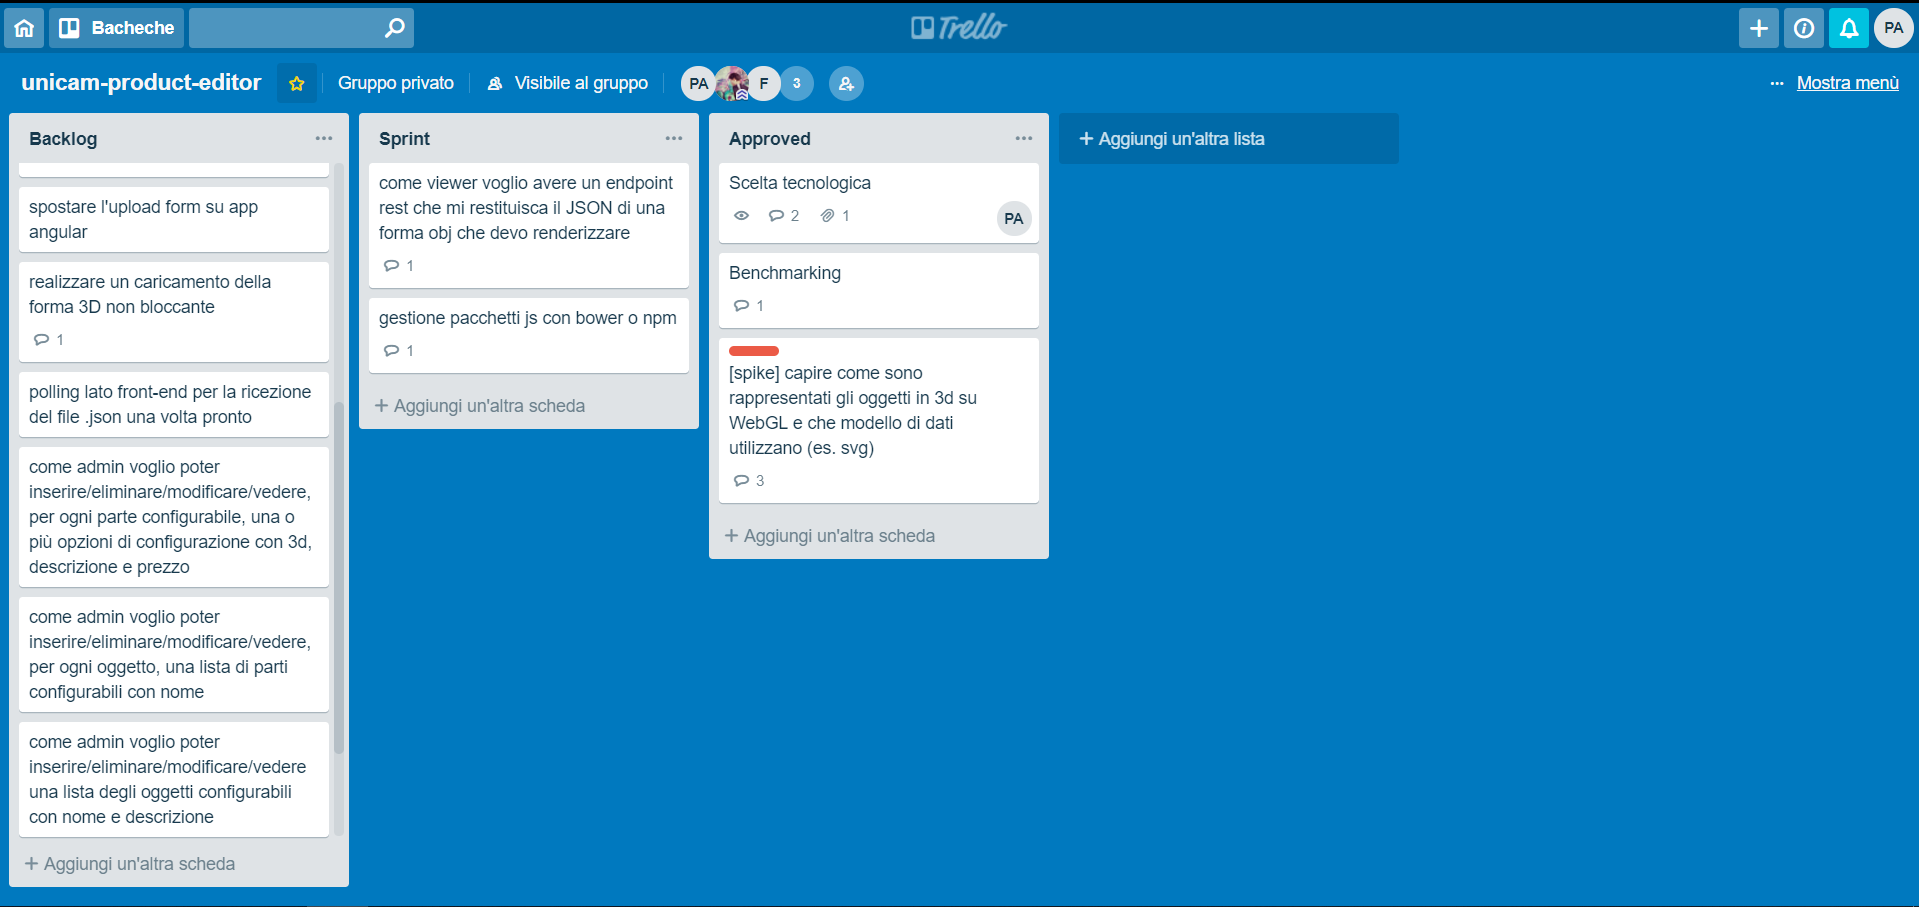
\includegraphics[scale=0.35]{Immagini/trello_start.png} 
	\caption{Organizzazione di unicam-product-editor su Trello}
\end{figure}

\section{Analisi}
Si vuole realizzare una applicazione web che permetta di gestire gli oggetti 3D tramite upload, modifica e visualizzazione in formato .JSON.
Il backend deve ricevere in input una forma 3D sotto forma di file in formato .obj, convertirlo in .JSON e fornire i servizi REST\index{REST}.
Un utente deve poter inserire l'oggetto 3D tramite l'uploader, modificare i metadati dell'oggetto convertito e visualizzare il file convertito attraverso un apposito endpoint una volta effettuata l'autenticazione.
Il processo di upload e conversione in particolare non deve essere bloccante, in quanto l'utente deve poter continuare ad utilizzare il servizio anche durante l'upload di una forma 3D molto grande.

La struttura dei documenti all'interno del progetto sarà la seguente:
\begin{itemize}
	\item[$\bullet$] Lista
	\begin{itemize}
		\item[$\bullet$] Oggetto
		\item[$\cdot$] Omino Lego
		\begin{itemize}
			\item[$\bullet$] Parte
			\item[$\cdot$] Testa
			\item[$\cdot$] Busto
			\begin{itemize}
				\item[$\bullet$] Opzione
				\item[$\cdot$] Busto standard
				\item[$\cdot$] Busto con papillon
				\item[$\cdot$] Busto con cravatta
			\end{itemize}
		\end{itemize}
	\end{itemize}
\end{itemize}

Le user stories derivanti da questo processo di analisi verranno identificate dalla sigla "US-XX", in cui XX rappresenta un numero progressivo, e vengono elencate di seguito:

\begin{longtable}{|c|l|}
	% intestazione iniziale
	\hline
	\multicolumn{1}{|c|}{\textbf{Numero}} & \multicolumn{1}{c|}{\textbf{Descrizione}} \\
	\endfirsthead
	% intestazione normale
	\multicolumn{2}{l}{\footnotesize\itshape\tablename~\thetable:
		continua dalla pagina precedente} \\
	\hline
	\multicolumn{1}{|c|}{\textbf{Numero}} & \multicolumn{1}{c|}{\textbf{Descrizione}} \\
	\endhead
	% piede normale
	\multicolumn{2}{r}{\footnotesize\itshape\tablename~\thetable:
		continua nella prossima pagina} \\
	\endfoot
	% piede finale
	\multicolumn{2}{r}{} \\
	\endlastfoot
	\hline
	US-01 & Scelta tecnologica.\\
	\hline
	US-02 & Benchmarking.\\
	\hline
	US-03 & Capire come sono rappresentati gli oggetti in 3d su WebGL e che\\ 
	& modello di dati utilizzano (es. svg).\\
	\hline
	US-04 & Come admin voglio poter inserire/eliminare/modificare/vedere una\\
	& lista degli oggetti configurabili con nome e descrizione.\\
	\hline
	US-05 & Come admin voglio poter inserire/eliminare/modificare/vedere,\\  & per ogni oggetto, una lista di parti configurabili con nome.\\
	\hline
	US-06 & Come admin voglio poter inserire/eliminare/modificare/vedere,\\  & per ogni parte configurabile, una o più opzioni di configurazione\\ & con 3D, descrizione e prezzo.\\
	\hline
	US-07 & Come viewer voglio avere un endpoint rest che mi restituisca\\   & il JSON di una forma obj che devo renderizzare.\\
	\hline
	US-08 & Creare app single-page con Angular.\\
	\hline
	US-09 & Realizzare un caricamento della forma 3D non bloccante\\ & (upload, conversione ed endpoint in modo sincrono).\\
	\hline
	US-10 & Polling lato front-end per la ricezione del file .JSON una volta pronto.\\
	\hline
	\caption{User stories}
	\label{tab:user:sto} \\
\end{longtable} 

Il diagramma di Gantt riguardante l'assegnazione dei task e lo svolgimento temporale, è il seguente:
\begin{figure}[h]
	\centering
	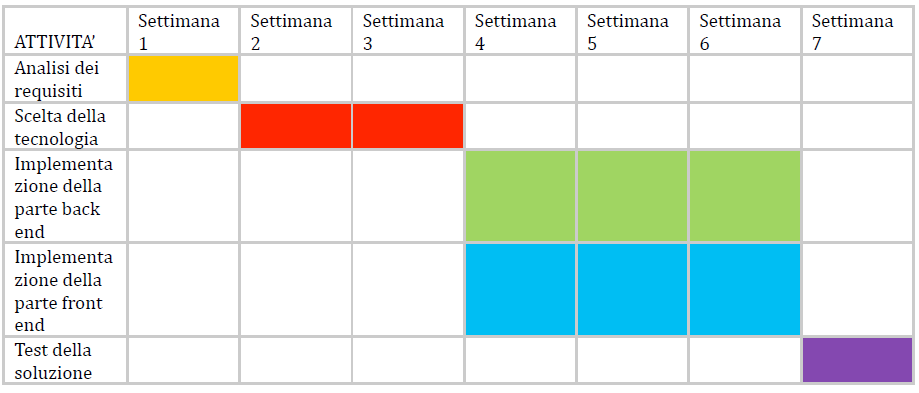
\includegraphics[scale=0.7]{Immagini/piano_realizzazione_progetto.png}
	\caption{Piano di realizzazione del progetto}
\end{figure}
\chapter{E-commerce}
\label{chap:ecommerce}
In questo capitolo si illustrano brevemente le tecnologie di visualizzazione applicate nell' e-commerce, oltre alle tecnologie di 3D e di Realtà Aumentata.

\section{Visualizzazione dei prodotti nell'e-commerce}
Foto, grafica 360 (comunque foto), configuratori basati su fotografie

\section{3D e realtà aumentata}
Il 3D e la realtà aumentata (nell'ecommerce)
\chapter{Scelta Tecnologica}
\label{chap:scelta}
In questo capitolo viene trattata l'architettura utilizzata per unicam-product-editor e il modo in cui vengono gestiti i dati attraverso la web app, per poi passare ad illustrare l'organizzazione del codice.

Per sviluppare unicam-product-editor è stato utilizzato lo stack MEAN\index{MEAN} che non è altro che l'insieme dei quattro componenti che ne fanno parte:
\begin{itemize}
	\item M = MongoDB: il popolare database
	\item E = Express.js: un framework web leggero
	\item A = Angular.js: un framework per la creazione di single page application
	\item N = Node.js v4: un interprete JavaScript costruito sul motore JavaScript V8 di Google Chrome orientato agli eventi che lo rende efficiente e leggero
\end{itemize}
Lo stack MEAN è un' alternativa al più tradizionale stack LAMP\index{LAMP} (Linux, Apache, MySQL, PHP/Perl/Python/P…), molto popolare per il suo utilizzo nella costruzione di applicazioni web dagli anni '90 in poi.
Di seguito andiamo a costruire le RESTful API, che sono la base per qualsiasi tipo di applicazione, come un sito web, un'app Android, iOS o Ubuntu Touch.

\section{Oggetti 3D}
Un modello 3D è una rappresentazione matematica di un oggetto tridimensionale e consiste sostanzialmente in un file di dati strutturati, contenenti le proprietà delle primitive geometriche che costituiscono l'oggetto rappresentato (un corpo fisico). Un oggetto 3D quindi non è altro che un insieme di dati composto da punti nello spazio tridimensionale (tre dimensioni X, Y e Z) e altre informazioni (spesso metadati, o informazioni aggiuntive).
I principali formati utilizzati per i modelli 3D:
\begin{itemize}
	\item OBJ
	\item FBX
	\item Collada
	\item BLEND
	\item DFX
	\item STL
	\item PLY
	\item 3DS (obsoleto)
	\item VRML (obsoleto)
	\item X3D
\end{itemize}
La scelta per cui abbiamo optato per la realizzazione del nostro progetto è ricaduta sul .obj, o più correttamente Wavefront .obj\index{obj}, un formato di file sviluppato dalla Wavefront Technologies per il software Advanced Visualizer. Il motivo di questa scelta risiede nel fatto che il .obj è un formato aperto che è stato adottato da tantissimi applicativi per la grafica 3D per l'interscambio di dati con altri programmi; ciò lo rende perfetto per il nostro progetto, in quanto questo dovrà poi essere trasformato in un corrispondente file .JSON per poter essere interpretato dal viewer\index{unicam-product-viewer}.

Questo è, per intero, il file .obj per la creazione di un cubo

\begin{lstlisting}[caption={Cube.obj}, style=JavaScriptCode]
# cube.obj
#

g cube

v  0.0  0.0  0.0
v  0.0  0.0  1.0
v  0.0  1.0  0.0
v  0.0  1.0  1.0
v  1.0  0.0  0.0
v  1.0  0.0  1.0
v  1.0  1.0  0.0
v  1.0  1.0  1.0

vn  0.0  0.0  1.0
vn  0.0  0.0 -1.0
vn  0.0  1.0  0.0
vn  0.0 -1.0  0.0
vn  1.0  0.0  0.0
vn -1.0  0.0  0.0

f  1//2  7//2  5//2
f  1//2  3//2  7//2 
f  1//6  4//6  3//6 
f  1//6  2//6  4//6 
f  3//3  8//3  7//3 
f  3//3  4//3  8//3 
f  5//5  7//5  8//5 
f  5//5  8//5  6//5 
f  1//4  5//4  6//4 
f  1//4  6//4  2//4 
f  2//1  6//1  8//1 
f  2//1  8//1  4//1 
\end{lstlisting}
in cui sono specificate le posizioni e le grandezze nello spazio tridimensionale dei vertici (v), dei vertici normali (vn), e delle facce (f).

\newpage
L'oggetto 3D che ne deriva può essere facilmente visualizzato tramite ad esempio il programma Paint 3D:

\begin{figure}[h]
	\centering
	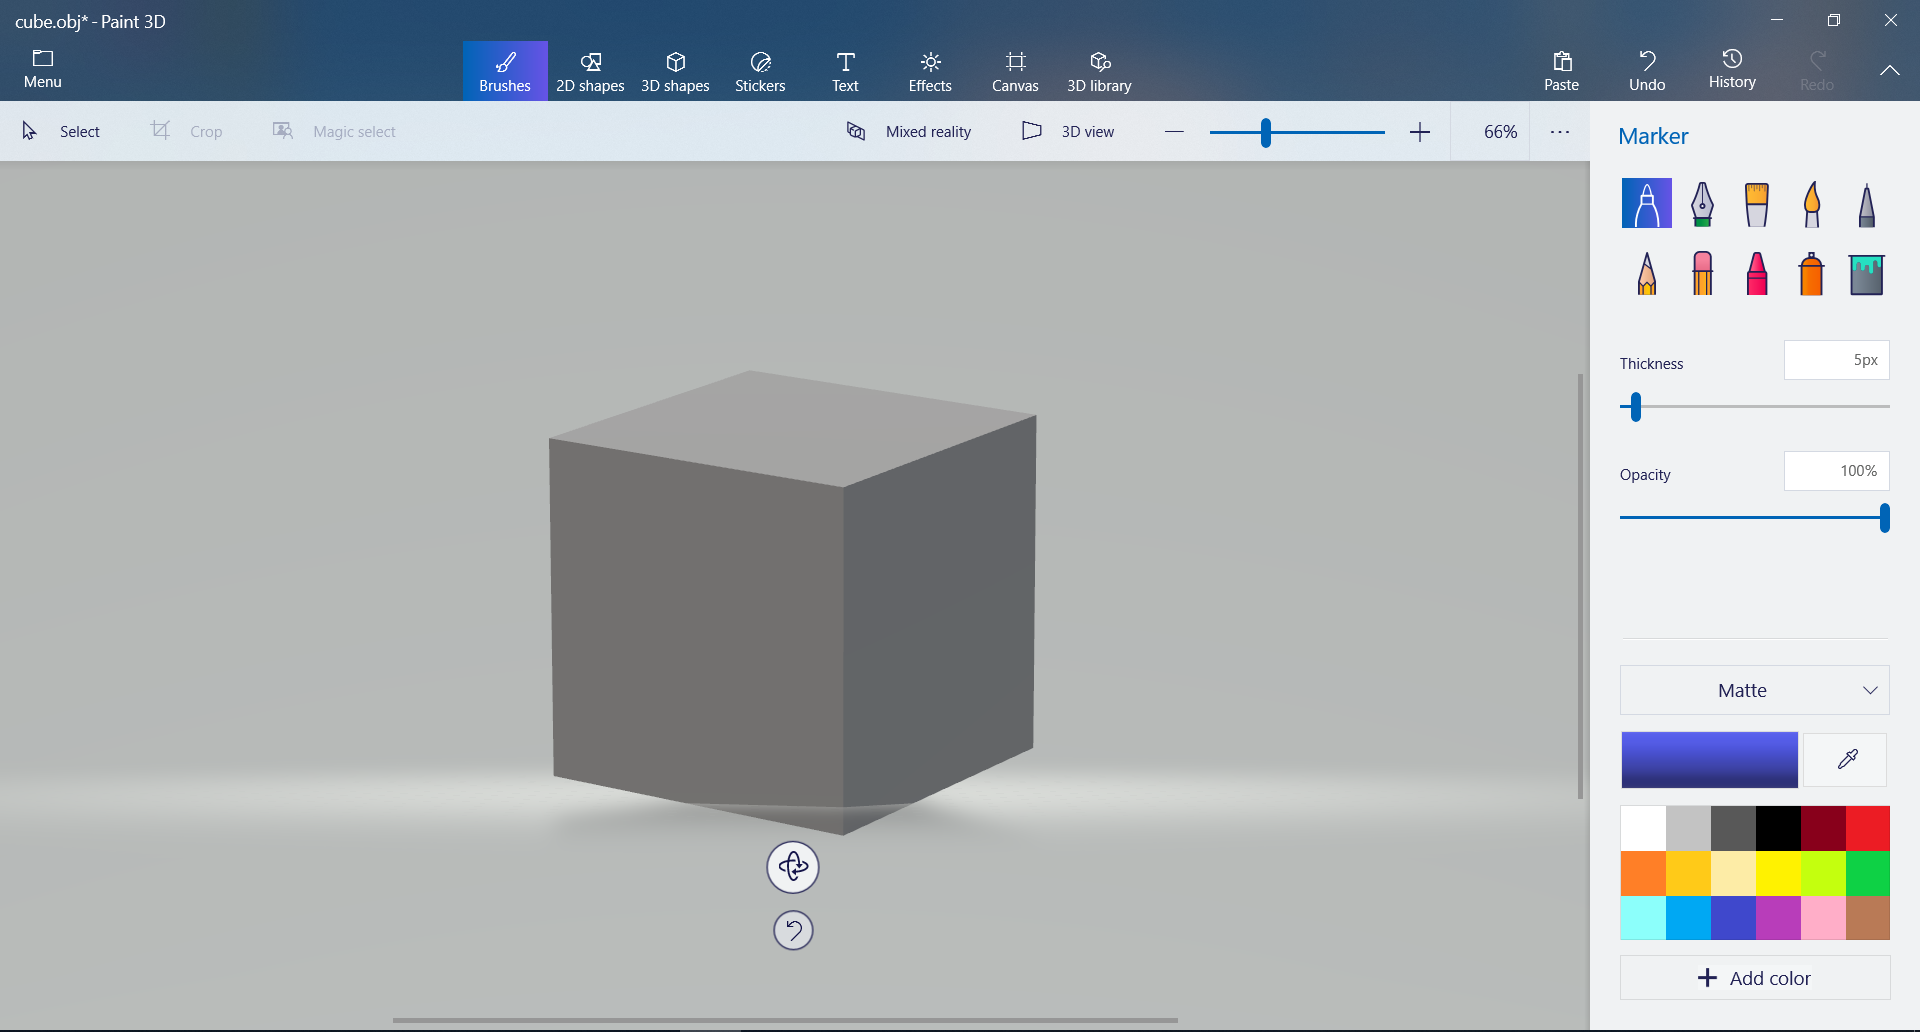
\includegraphics[scale=0.35]{Immagini/cube_obj.png}
	\caption{Visualizzazione grafica di cube.obj}
\end{figure}

\section{JSON}
JSON è un formato di dati molto leggere basato su un sottoinsieme della sintassi JavaScript, cioè \emph{array literal} e \emph{object literal}, proposto da Douglas Crockford come formato per i servizi web in sostituzione al verboso XML\index{XML}.

Dato l'utilizzo della sintassi Javascript, le definizioni JSON\index{JSON} possono essere incluse all'interno dei file JavaScript\index{JavaScript}.
\subsection{Gli array literal}

Gli \emph{array literal} rappresentano il metodo più semplice per creare un array in JavaScript.
Basta infatti elencare una insieme di valori separati da una virgola all'interno delle parentesi quadre, per esempio:
\begin{lstlisting}[style=JavaScriptCode]
var users = ["Paolo", "Antonio", "Filippo"];
\end{lstlisting}
A livello di programmazione è equivalente al codice:
\begin{lstlisting}[style=JavaScriptCode]
var users = new Array("Paolo", "Antonio", "Filippo");
\end{lstlisting}
Entrambe le definizioni generano lo stesso risultato ed è possibile accedere ad ogni elemento dell'array utilizzando il relativo indice 
\begin{lstlisting}[style=JavaScriptCode]
console.log(users[0]); \\prints Paolo 
console.log(users[1]); \\prints Antonio
console.log(users[2]); \\prints Filippo
\end{lstlisting}
Gli array in JavaScript hanno però due caratteristiche ben precise:
\begin{enumerate}
	\item In JavaScript l'array non ha un tipo di dati ben definito (non è tipizzato), e quindi ogni elemento può contenere tipi di dati diversi.
	\item Nonostante entrambi i metodi sopra citati per la creazione di un array siano validi in JavaScript, in .JSON soltanto gli array literal verranno accettati e interpretati correttamente.
\end{enumerate}

\subsection{Gli object literal}
Un object literal è definito tra parentesi graffe.
Al suo interno troviamo un numero qualsiasi di coppie chiave-valore, definite con una stringa, i due punti ed il valore.
Ogni coppia deve essere seguita da una virgola, tranne l'ultima. 
Questo insieme di coppie chiave-valore rappresenta, nel suo insieme, un oggetto.
Un esempio:
\begin{lstlisting}[style=JavaScriptCode]
var user = {
"firstname": "Paolo",
"age": 23,
"student": true
};
\end{lstlisting}
Il codice qui sopra genera un oggetto \emph{user} con le proprietà firstname, age e student. 
Per accedere alle proprietà dell'oggetto basta usare la notazione con il punto:
\begin{lstlisting}[style=JavaScriptCode]
console.log(user.firstname); \\prints "Paolo"
console.log(user.age); \\prints "23"
console.log(user.student); \\prints "true"
\end{lstlisting}
Lo stesso oggetto potrebbe essere creato utilizzando il costruttore \texttt{Object} di JavaScript
\begin{lstlisting}[style=JavaScriptCode]
var user = new object():
user.firstname = "Paolo";
user.age = 23;
user.student = true;
\end{lstlisting}
Come già detto, sebbene entrambe le definizioni siano accettate in JavaScript, in JSON è valida solo la seconda notazione, object literal.
\subsection{La sintassi JSON}
La sintassi di JSON non è altro che il miscuglio di object literal ed array literal per memorizzare dati e solo e soltanto rappresentarli.
Un esempio:
\begin{lstlisting}[style=JavaScriptCode]
[
{
"firstname": "Paolo",
"age": 23,
"student": true
},
{
"firstname": "Giuseppe",
"age": 40,
"student": false
}
]
\end{lstlisting}
La prima cosa da notare è che in questo documento non sono presenti variabili, così come punti e virgola.
In questo modo quando si trasmettono dei dati tramite HTTP ad un browser, il tutto avviene abbastanza velocemente grazie al numero ridotto di caratteri.

Oltre a questo, ci sono altri ovvi benefici nell'utilizzo di JSON come formato dati per la comunicazione in JavaScript: non bisogna preoccuparsi della valutazione dei dati, e quindi, è garantito un accesso più veloce alle informazioni che questo contiene.



\section{RESTful API}
Il significato dell’acronimo REST è REpresentational State Transfer, ossia una rappresentazione del trasferimento di stato di un determinato dato.

REST utilizza un modello client-server, dove il server è un server HTTP e il client invia richieste HTTP (GET, POST, PUT, DELETE), con un URL che al suo interno contiene i parametri codificati. L'URL descrive l'oggetto e il server genericamente risponde restituendo un'immagine, un documento HTML, un file CSV o qualunque altro tipo di dato.
Nel nostro caso il server risponde restituendo del codice e un JSON (JavaScript Object Notation).
Una RESTful API quindi è l'Interfaccia di Programmazione di un'Applicazione che usa le richieste HTTP per gestire i dati che vengono scambiati fra client e server.

Dato che in unicam-product-editor viene utilizzato lo stack MEAN, abbiamo scelto di utilizzare documenti JSON che risultano particolarmente adatti per la nostra applicazione, visto che tutti i nostri componenti sono in JavaScript e MongoDB interagisce perfettamente con questo formato. 
Faremo degli esempi più dettagliati più avanti quando definiremo i nostri Data Model.

Le operazioni principali che si possono eseguire con questo metodo sono le seguenti:
\begin{itemize}
	\item\texttt{GET} per richiedere al server un determinato set di dati;
	\item\texttt{POST} per creare un nuovo documento all’interno del database;
	\item\texttt{PUT} per modificare o sostituire completamente un documento già esistente;
	\item\texttt{DELETE} per cancellare un documento contenuto all’interno del database al quale siamo collegati. 
\end{itemize}

Queste operazioni vengono spesso descritte attraverso l'acronimo CRUD, che sta per CREATE, READ, UPDATE e DELETE.
Il server HTTP, da parte sua, usa spesso assieme alle API REST dei codici di risposta; di seguito vengono elencati alcuni fra i più comuni:
\begin{itemize}
	\item 200 - “OK”
	\item 201 - “Created” (Utilizzato con POST)
	\item 400 - “Bad Request” (Ad esempio per l'assenza di parametri)
	\item 401 - “Unauthorized” (Non ci sono i parametri per l'autenticazione)
	\item 403 - “Forbidden” (L'utente è autenticato ma non ha i permessi)
	\item 404 - “Not Found”
\end{itemize}
Una descrizione completa è contenuta nell'apposito RFC 2616\cite{RFC2616}.

Lo sviluppo di API REST è alla base del nostro sviluppo, in quanto permette alla nostra applicazione di essere multipiattaforma. Per fare alcuni esempi di applicazioni di questo tipo si possono citare Google Docs, Pixlr o lo stesso Trello insieme ad Evernote. Le API REST permettono la facile implementazione dell'applicazione su molte piattaforme che potranno essere sviluppate in un secondo momento, trasformando il progetto iniziale in un progetto indipendente dalla piattaforma di partenza.

I dati da gestire nel nostro progetto si possono riassumere in questo modo:
\begin{itemize}
	\item Dati degli utenti
	\item Liste
	\item Oggetti
	\item Opzioni di ogni oggetto
	\item Parti di ogni opzione
\end{itemize}
Come potremo vedere a breve, diversamente dai tradizionali Database relazionali (in cui la forma principale di struttura dati è data dalle Tabelle), in MongoDB, essendo un Database NoSQL, e quindi non relazionale, non si parla di Tabelle, anche se il concetto di Database ad alto livello è lo stesso.

Nel Database MongoDB possono essere contenute più Collection, che possono forse essere paragonate alle Tabelle nei Database relazionali. A sua volta, ogni Collection conterrà uno o più Document, che a confronto con un Database relazionale corrisponde all'incirca alla riga di una Tabella. Ogni Document (così come ogni Collection) non segue però uno schema specifico come in una Tabella, ma può essere formato da una o più coppie chiave-valore, dove il contenuto può essere a sua volta una variabile semplice oppure qualcosa di più complicato come un array.

Il documento JSON appena preso in esempio rappresenta un utente nel nostro sistema. Ogni campo ha il suo specifico scopo, ma il campo più importante in un Document MongoDB è senza dubbio il campo \texttt{\_id}: questo rappresenta la chiave primaria di ogni Document. Quando un Document viene salvato senza questo campo, MongoDB ne assegna uno automaticamente, e con un valore univoco.

Ora passiamo ai vari Document che compongono le nostre Collection; la Collection degli Utenti conterrà Documenti di questo tipo:
\begin{lstlisting}[caption={User Collection}, style=javaScriptCode]
{
	"_id": {
		"$oid": "5894fa05f882a91c7c5cf0e6"
	},
	"displayName": "Paolo Andreassi",
	"email": "pablo15941@gmail.com",
	"password": "$2a$10$kyaJc1WP9KFvSVWzrPagLe.vgY76FjBQjwt76.HhC5u9oo96qoRo.",
	"__v": 0,
	"picture": "https://graph.facebook.com/v2.3/10209758034881202/...",
	"google": "106815394034042298036"
}
\end{lstlisting}
Si può notare l'importante presenza del campo \texttt{\_id}, così come gli altri dati utili al riconoscimento dell'utente. La password inoltre in unicam-product-editor non viene mai mostrata in chiaro all'interno del Database, anche se il campo ad essa corrispondente è presente e popolato. Questo è il risultato di una password impostata dall'utente ma successivamente encriptata con una funzione hash.
\newpage
Il Document di tipo Lista ha uno scopo puramente descrittivo nei confronti di ciò che contiene:
\begin{lstlisting}[caption={List Collection}, style=javaScriptCode]
{
"_id": {
"$oid": "589a30d1b2a4c717a8da16b3"
},
"nome": "Omino LEGO",
"__v": 0
}
\end{lstlisting}

La Collection degli Oggetti avrà dei Document in cui i campi \texttt{nome} e \texttt{descrizione} hanno una funzione descrittiva, ma oltre al campo \texttt{\_id} è presente il campo \texttt{\_list} che funge da collegamento con la Collection delle Liste: in questo campo infatti è indicato l'identificativo della Lista a cui appartiene uno specifico Oggetto:
\begin{lstlisting}[caption={Object Collection}, style=javaScriptCode]
{
"_id": {
"$oid": "589a38f93ec83413e4f010b2"
},
"nome": "Omino LEGO",
"descrizione": "LEGO figure",
"_list": [
"589a30d1b2a4c717a8da16b3"
],
"__v": 0
}
\end{lstlisting}

Essendo un Database con una struttura nidificata, anche i Document nelle Collection delle Parti e delle Opzioni avranno una struttura simile a quelli delle Collection degli Oggetti: anche in queste infatti è indicato il campo del Documento \emph{parente} a cui fanno riferimento:
\begin{lstlisting}[caption={Part Collection}, style=javaScriptCode]
{
"_id": {
"$oid": "589a3a2857ba982460b83fb7"
},
"nome": "Testa",
"_object": [
"589a38f93ec83413e4f010b2"
],
"__v": 0
}
\end{lstlisting}

La differenza più importante risiede nei Document che compongono la Collection delle Opzioni: in questi vengono indicati anche il campo \texttt{prezzo}, ma soprattutto il campo \texttt{forma}, che contiene una parte di URL con cui effettuare una chiamata REST API. Il campo forma, che viene mostrato all'utente nell'interfaccia della applicazione web, permette di visualizzare il file JSON relativo ad una forma 3D inserita tramite l'uploader e successivamente convertita nel formato usato da MongoDB e JavaScript:
\begin{lstlisting}[caption={Option Collection}, style=javaScriptCode]
{
"_id": {
"$oid": "589a3c5938319d1c8cb4e787"
},
"nome": "Testa Yoda",
"prezzo": 50,
"forma": "/shape/58593a6319290c09984a439b",
"_part": [
"589a3a2857ba982460b83fb7"
],
"__v": 0
}
\end{lstlisting}

Infine la Collection delle forme 3D convertite contiene l'insieme dei file JSON che rappresentano le stesse forme.

\section{Documentazione}
Una parte fondamentale della progettazione di API REST è la documentazione.
Per scrivere la documentazione necessaria è stato usato lo strumento Postman.

Postman\index{Postman} è un ambiente di sviluppo multipiattaforma utile per testare le API, ossia per eseguire una qualsiasi chiamata HTTP al nostro server, e monitorare la risposta ottenuta in modo chiaro e leggibile. 
Tramite questo strumento è possibile effettuare delle chiamate API senza dover mettere mano al codice dell’applicazione, consentendo di effettuare le chiamate tramite questo plugin che fornisce un’utile interfaccia grafica. Le richieste possono essere effettuate sia verso un server locale che verso un server online impostando tutti i dati di una tipica chiamata API, dagli headers al body.
\begin{figure}[h]
	\centering
	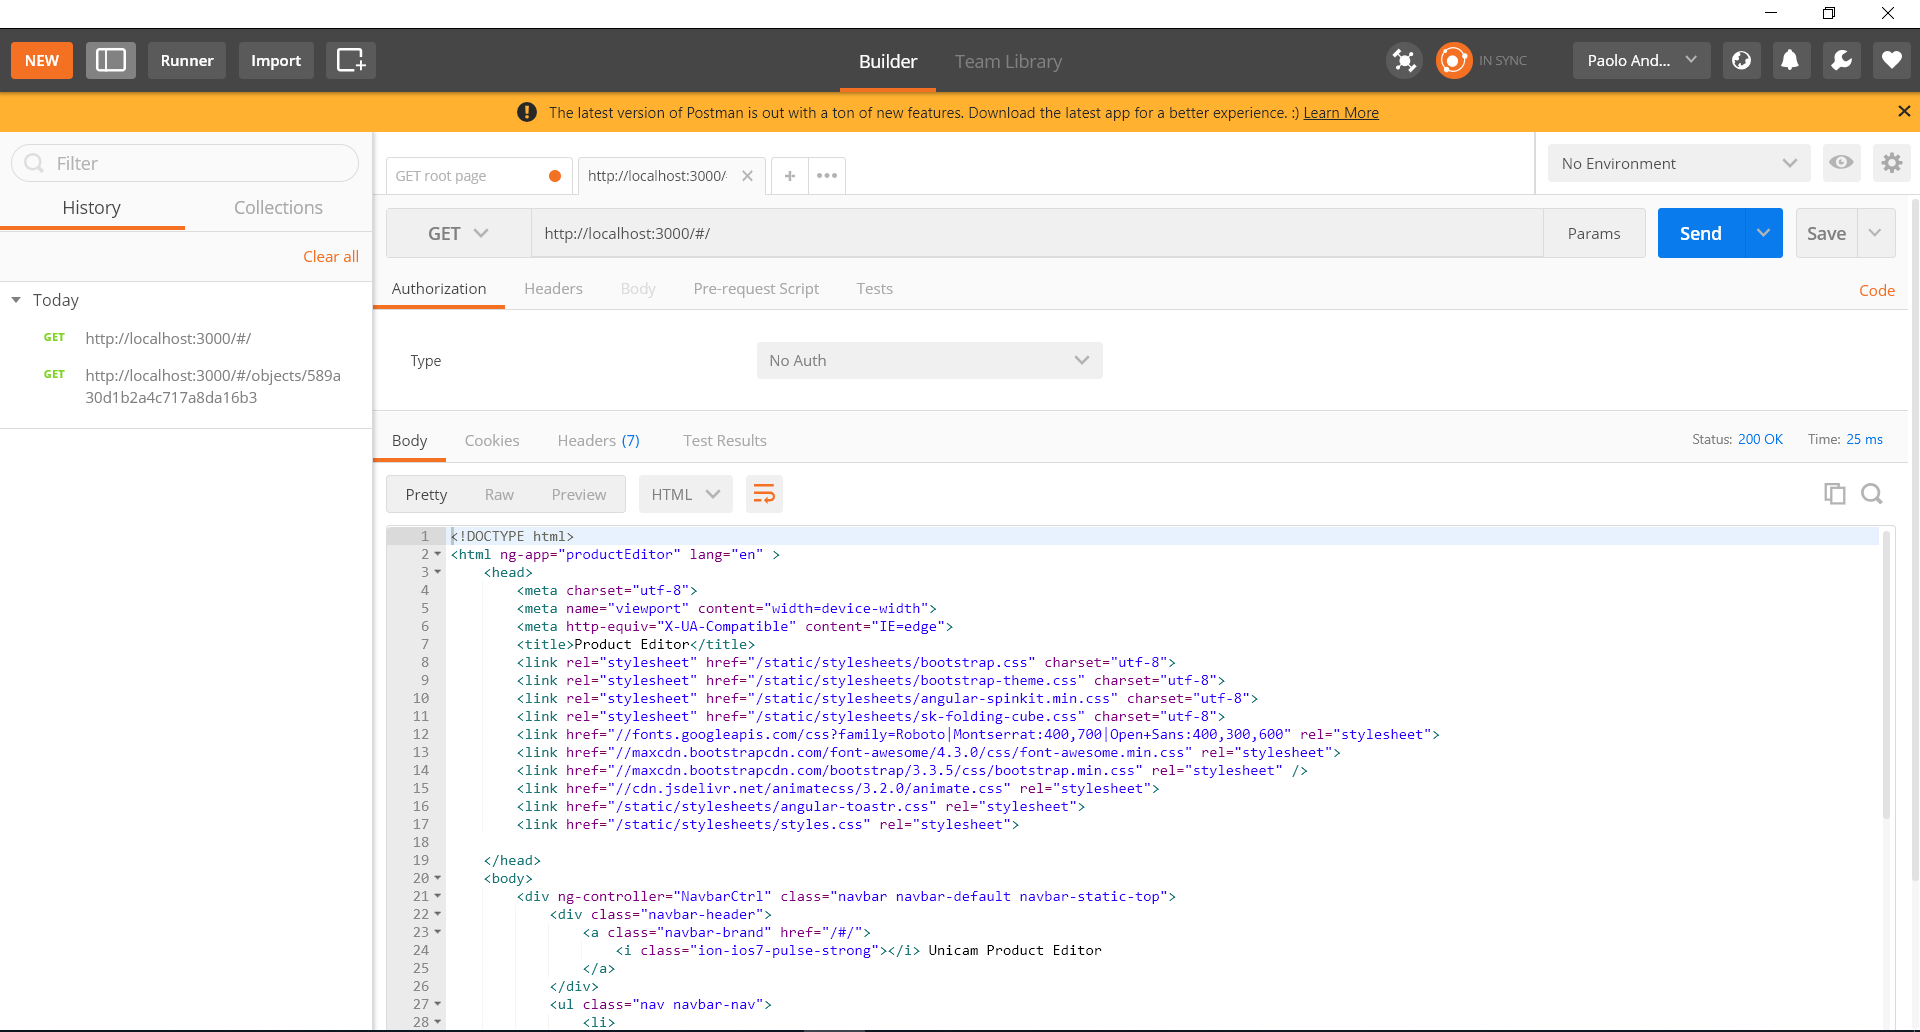
\includegraphics[scale=0.35]{Immagini/postman_ui.png}
	\caption{L'interfaccia utente di Postman}
\end{figure}

\section{NodeJS}
Node.js\cite{node}\index{Node} v4 è un interprete JavaScript orientato agli eventi, progettato per realizzare applicazioni di rete scalabili.
La caratteristica principale è che rimane inattivo finché non arriva una connessione in ingresso, o più generalmente un qualsiasi evento, e viene chiamata la relativa callback.
Questo paradigma è in contrasto con quello tradizionale basato sui thread.
Il principale vantaggio del paradigma ad eventi rispetto a quello basato sui thread si ha quando c'è un alto traffico.
In questo caso, infatti, l'alto numero di thread genera un alto overhead diminuendo drasticamente le prestazioni della macchina host.
Inoltre, dato che nessuna funzione di Node eseguirà direttamente operazioni di I/O, il processo non si bloccherà mai.

La versione di Node usata in unicam-product-editor è la v4.6.0.
Se da un lato su un server è normale avere solo una versione di Node, potrebbe non esserlo su una macchina di sviluppo.
Può capitare, infatti, che uno sviluppatore sia impegnato su più progetti Node che utilizzano versioni differenti.
Per risolvere questo problema possiamo installare NVM\index{NVM}.
Node Version Manager permette di avere più versioni di Node contemporaneamente nel nostro sistema e fornisce una semplice CLI per poterle gestire.
In particolare, basta creare un file di testo chiamato \texttt{.nvmrc} in cui salvare il numero di versione di Node che si intende usare per la cartella corrente.
Poi, sarà sufficiente digitare il comando \texttt{nvm install} per scaricare ed utilizzare la giusta versione.

Node è disponibile per diverse piattaforme, come Linux, Microsoft Windows e Apple OS X.
Le applicazioni Node.js vengono costruite utilizzando librerie e moduli disponibili per l'ecosistema ed alcuni di essi sono stati utilizzati in unicam-product-editor.
Per iniziare ad utilizzare Node.js, dobbiamo per prima cosa creare un file \texttt{package.json}, che descrive la nostra applicazione ed elenca tutte le sue dipendenze.
NPM (Node.js Package Manager)\index{NPM} installa una copia delle librerie in una sotto-cartella chiamata \texttt{node\_modules/}, della cartella principale dell'applicazione. 
Questo comporta diversi benefici, ad esempio isola le diverse versioni delle librerie, evitando così i problemi di compatibilità che si sarebbero presentati se avessimo installato tutto in una cartella standard come \texttt{/usr/lib}.

Il comando \texttt{npm install} creerà la cartella \texttt{node\_modules/}, con dentro tutte le librerie richieste e specificate nel file package.json:

\begin{lstlisting}[caption={package.json}, style=javaScriptCode][h]
{
	"name": "unicam-product-editor",
	"version": "1.0.0",
	"private": "true",
	"description": "Editor di prodotti 3D",
	"repository": "https://github.com/e-xtrategy/unicam-product-editor",
	"main": "app.js",
	"scripts": {
		"test": "nodemon --ignore tmp/ app.js",
		"start": "node app.js"
	},
	"author": "Paolo Andreassi",
	"license": "ISC",
	"dependencies": {
	...
	"async": "^2.1.4",
	"bcryptjs": "^2.4.0",
	"body-parser": "^1.15.2",
	...
	"cors": "^2.8.1",
	"express": "^4.14.0",
	"express-fileupload": "0.0.5",
	"express-handlebars": "^3.0.0",
	...
	"mongodb": "^2.2.10",
	"mongoose": "^4.7.8",
	...
	"python-shell": "^0.4.0",
	...
	"satellizer": "^0.15.5",
	...
	},
	"devDependencies": {
		"nodemon": "^1.11.0",
		"should": "~7.1.0",
		"supertest": "~1.1.0"
	},
		"engines": {
		"node": "4.6.0"
	}
}
\end{lstlisting}

E' interessante analizzare alcune parti di questo file, oltre al fatto che anche questo è in formato JSON, e oltre alle prime righe che descrivono il progetto in sé per sé.
Ci sono due script: quello chiamato \emph{start} avvia l'applicazione normalmente tramite il comando \texttt{node} seguito dal nome del file principale del server \texttt{app.js}.
Lo script chiamato \emph{test} invece è interessante, perché avvia uno strumento (installato tramite l'apposita dipendenza) chiamato nodemon. Questo utilissimo \emph{demone} fa sì che in fase di test ogni qual volta si verifichi un errore che interrompe l'esecuzione del server nodemon attende un salvataggio dei file del progetto, che indica che lo sviluppatore ha modificato il codice per correggere l'errore, e non appena questo evento si verifica il demone riavvia in automatico il server ricominciando ad eseguire il codice.

Un'altra dipendenza interessante riguarda \emph{python-shell}, che nel nostro progetto servirà ad eseguire lo script della libreria Three.js scritto in codice Python (altrimenti non eseguibile da Javascript), che si occupa di convertire il file .obj in JSON. python-shell può ricevere in input interi file scritti in Python per eseguirli in modo asincrono.

\section{Configurazione iniziale e Test}
Andiamo ora ad analizzare l'inizializzazione di un server Node.js, la configurazione di MongoDB su Mongolab e l'interazione di questi attraverso Express e Mongoose, che sono elementi che vedremo comunque più tardi.

Il primo comando che si utilizza per inizializzare il progetto e per creare il relativo file package.json è \texttt{npm init}. Il comando va lanciato dalla root del progetto, che sarà collegata al repository su GitHub.
Il prossimo passo consiste nel creare il file JavaScript del server in sé per sé. Questo file in unicam-product-editor si chiama \texttt{app.js}, ed è contenuto anch'esso nella root del progetto. Per eseguire già da ora il server, basterà posizionarsi con il prompt dei comandi nella root del progetto e lanciare il comando \texttt{node} seguito dal nome del file del server appena creato, quindi \texttt{node app.js}.

Si passa ora ad importare il framework express tramite la sua dipendenza e usando il gestore di pacchetti NPM. Per fare ciò dal prompt dei comandi basterà eseguire lo script \texttt{npm install express --save}. L'opzione \texttt{--save} serve a far comparire la dipendenza appena installata nell'apposita sezione del file package.json. Dalla versione 5.0.0 di NPM comunque questo comando è implicito.
Alla fine dell'esecuzione dello script, avremo la dipendenza installata localmente nella cartella \texttt{node\_modules/}, e il file package.json apparirà come segue:

\begin{lstlisting}[caption={test installazione express}, style=javaScriptCode]
{
	"name": "node server",
	"version": "1.0.0",
	"main": "app.js",
	"author": "Paolo Andreassi",
	"license": "ISC",
	"dependencies": {
	...
	"express": "^4.14.0",
	...
	}
}

\end{lstlisting}
Di conseguenza, andremo ad utilizzare express nel nostro file \texttt{app.js} come segue:
\begin{lstlisting}[caption={test require express}, style=javaScriptCode]
const express = require('express');
const app = express();
\end{lstlisting}
e lo utilizzeremo subito per creare il nostro server in ascolto sulla porta 3000 (almeno per questo test) tramite l'apposita istruzione
\begin{lstlisting}[caption={test server express}, style=javaScriptCode]
app.listen(3000, function() {
	console.log('listening on port 3000')
})
\end{lstlisting}
In express possiamo gestire le richieste HTTP GET attraverso il metodo \texttt{get}:
\begin{lstlisting}[style=javaScriptCode]
app.get(path, callback)
\end{lstlisting}
che useremo così per la nostra configurazione di test
\begin{lstlisting}[caption={test hello world}, style=javaScriptCode]
app.get('/', function(req, res) {
	res.send('Hello World')
})
\end{lstlisting}
In questo modo aprendo il nostro browser e digitando \texttt{localhost:3000} nella barra URL, dopo esserci assicurati di aver avviato l'applicazione, quello che il nostro server risponderà alla richiesta HTTP GET sarà:
\begin{figure}[h]
	\centering
	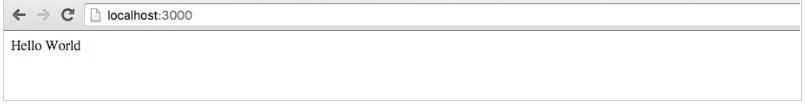
\includegraphics[scale=0.8]{Immagini/test_hello_world.png}
	\caption{Test di una richiesta HTTP GET}
\end{figure}

Una volta configurato il server per questo test, andiamo a fare lo stesso per il nostro database MongoDB.
In unicam-product-editor il database è ospitato in cloud attraverso il servizio mLab\index{mLab}, che a sua volta si appoggia a servizi cloud quali Amazon Web Services, Google Cloud Platform e Windows Azure. mLab offre diversi piani tariffari, ma per il nostro progetto il piano Sandbox che offre 0.5GB di spazio gratuito va più che bene. Una volta creato il database su mLab, e dopo aver creato un utente di tipo amministratore per lo stesso database, mLab creerà una indirizzo URL, detto MongoDB URI, utilizzabile per connettersi a questo servizio, mediante l'uso del nome utente e della password dell'account amministratore. 
\newpage
La stringa corrispondente al database di unicam-product-editor è la seguente:
\begin{figure}[h]
	\centering
	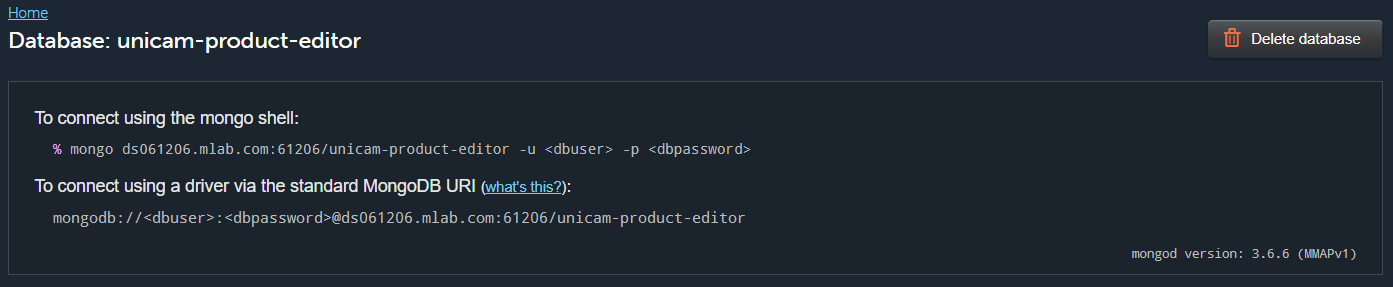
\includegraphics[scale=0.5]{Immagini/mongodb_uri.png}
	\caption{MongoDB URI}
\end{figure}

Come si può notare dalla schermata qui sopra, oltre ad essere indicata la versione del database in uso, è presente anche il comando da utilizzare per connettersi a mLab tramite il mongo shell, ossia un'interfaccia interattiva di MongoDB, che usa anch'essa istruzioni in JavaScript.
Il prossimo step consiste nell'utilizzare proprio questo MongoDB URI per connettersi al database. In questo caso di test useremo il client nativo mongodb, mentre in unicam-product-editor verrà utilizzata la libreria Mongoose, che vedremo più tardi.

Per installare il client mongodb basta lanciare il comando \texttt{npm install mongodb}, e per poterlo usare nel nostro progetto bisognerà importarlo come già fatto per Express, ossia tramite l'istruzione
\begin{lstlisting}[style=javaScriptCode]
const MongoClient = require('mongodb').MongoClient
\end{lstlisting}
L'istruzione standard in Express per la connessione al database tramite il client mongodb è la seguente:
\begin{lstlisting}[style=javaScriptCode]
MongoClient.connect('MONGODB_URI', function(err, client){
	...
})
\end{lstlisting}
e utilizzeremo la callback della funzione \texttt{.connect} per avviare il server Node.js solamente una volta che sarà avvenuta la corretta connessione al database. Per fare ciò basta aggiungere il codice
\begin{lstlisting}[caption={connessione a mongodb}, style=javaScriptCode]
MongoClient.connect('MONGODB_URI', function(err, client){
	if (err) return console.log(err)
	db = client.db('unicam-product-editor')
	app.listen(3000, function() {
		console.log('listening on port 3000')
	})
})
\end{lstlisting}
utilizzando la variabile db per salvare la sessione di collegamento al database appena ottenuta.

A questo punto la connessione al nostro database è pronta all'uso, e possiamo utilizzare la funzione \texttt{.collection} per gestire le Collection presenti nel database.
Se volessimo ad esempio inserire un Document in una Collection del database unicam-product-editor, la sintassi sarebbe la seguente:
\begin{lstlisting}[caption={mongodb save}, style=javaScriptCode]
db.collection('COLLECTION').save('DOCUMENT', function(err, result){
	if (err) return console.log(err) //in caso di errore

	console.log('saved to database') //in caso di corretto salvataggio
})
\end{lstlisting}

\section{Express}
Con express.js\index{Express}, noi abbiamo creato la vera e propria "applicazione", che ascolta le richieste HTTP in ingresso su una data porta. Quando arriva una richiesta, questa passa attraverso una catena di intermediari, detti \emph{middleware}.
Ogni nodo della catena è definito da un req (request) object, usato per ricevere dei parametri, e un res (results) object, usato per salvare i risultati. 
Ogni nodo può decidere se eseguire delle operazioni, o se passare i due oggetti al nodo successivo. 
Per aggiungere un nuovo middleware usiamo la funzione \texttt{app.use()}. 
Il middleware principale, chiamato “router”, analizza l’URL e il tipo di richiesta per poterla poi indirizzare verso una specifica funzione.

Il codice della nostra applicazione apparirà così organizzato, visto che i vari handler e le diverse funzioni specifiche saranno poi distribuiti in file separati.

\begin{lstlisting}[caption={app.js}, style=javaScriptCode]
var path = require('path'),
	qs = require('querystring'),

	async = require('async'),
	bcrypt = require('bcryptjs'),
	bodyParser = require('body-parser'),
	colors = require('colors'),
	cors = require('cors'),
	express = require('express'),
	exphbs = require('express-handlebars'),
	favicon = require('serve-favicon'),
	fileUpload = require('express-fileupload'),
	fs = require('fs'),
	http = require('http'),
	logger = require('morgan'),
	jwt = require('jwt-simple'),
	moment = require('moment'),
	mongoose = require('mongoose'),
	request = require('request'),
	url = require('url'),
	
	upload       = require('./app/upload'),
	convert      = require('./app/convert'),
	converted    = require('./app/converted'),
	readjsonfile = require('./app/readjsonfile'),
	users        = require('./routes/users'),
	getshapes    = require('./app/getshapes'),
	config       = require('./config');
	
var app = express();
app.set('port', process.env.NODE_PORT || 3000);
app.set('host', process.env.NODE_IP || 'localhost');
app.set('view engine', 'handlebars');
app.engine('handlebars', exphbs({defaultLayout: 'main'}));
app.use(bodyParser.json());
app.use('/static', express.static('public'));
app.use(express.static('partials'));
app.use(fileUpload());
require('./app/schema'),
require('./routes')(app);
\end{lstlisting}

e la route principale del progetto sarà così dichiarata, essendo Handlebars il motore di rendering utilizzato in unicam-product-editor:

\begin{lstlisting}[caption={configurazione server}, style=javaScriptCode]
app.get('/', function(req, res) {
	res.render('layouts/main.handlebars');
})
\end{lstlisting}

Handlebars.js\index{Handlebars} è un'estensione del linguaggio di template \emph{Mustache}, creato da Chris Wanstrath. Sia Handlebars.js che Mustache sono linguaggi di template \emph{logicless}, che tengono separate, come da convenzione, la parte visiva del progetto e la parte di codice, migliorando l'organizzazione del progetto stesso.

Per ultimo definiamo il nostro server in ascolto sulla porta indicata con la funzione Express \texttt{app.set(port)}, o sulla porta 3000 in tutti gli altri casi.
\begin{lstlisting}[caption={configurazione server}, style=javaScriptCode]
server = app.listen(process.env.PORT || 3000, function() {
	var port = server.address().port
	console.log("Express server listening on port %s", port)
})
\end{lstlisting}

\section{Mongoose}
A questo punto, i nostri dati vanno gestiti tramite l'uso di Mongoose\index{Mongoose}, un modellatore di oggetti MongoDB progettato per l'uso in Node.js.
Come detto in precedenza, le Collection da definire sono le seguenti:
\begin{itemize}
	\item Users
	\item Lists
	\item Objects
	\item Parts
	\item Shapes
\end{itemize}

Per fare ciò, bisogna definire uno schema per ognuna delle Collection appena esposte; partendo dal primo, lo UserSchema sarà così dichiarato:

\begin{lstlisting}[caption={userSchema}, style=javaScriptCode]
var userSchema = new mongoose.Schema({
	email: { type: String, unique: true, lowercase: true },
	password: { type: String, select: false },
	displayName: String,
	picture: String,
	facebook: String,
	google: String
});
\end{lstlisting}

come possiamo notare, con mongoose e MongoDB è possibile non solo dichiarare il tipo di dato che ogni proprietà conterrà, ma anche dei vincoli attraverso l'uso dei trim.
Inoltre con mongoose è possibile definire, all'interno dello userSchema, funzioni e metodi che potremo all'occorrenza richiamare da altre parti del progetto.

\begin{lstlisting}[caption={userSchema}, style=javaScriptCode]
userSchema.pre('save', function(next) {
	var user = this;
	if (!user.isModified('password')) {
		return next();
	}
	bcrypt.genSalt(10, function(err, salt) {
		bcrypt.hash(user.password, salt, function(err, hash) {
			user.password = hash;
			next();
		});
	});
});

userSchema.methods.comparePassword = function(password, done) {
	bcrypt.compare(password, this.password, function(err, isMatch) {
		done(err, isMatch);
	});
};
\end{lstlisting}

La funzione \texttt{userSchema.pre} viene eseguita appena prima dell'inserimento di un nuovo utente (tramite la funzione save) e si assicura di encriptare nuovamente la password di un utente ogni qual volta questa venga cambiata, prima di inserirla nel database.
Il metodo \texttt{.comparePassword} invece si avvale dell'uso della libreria \emph{bcrypt} per decriptare la password passata al metodo come parametro prima di confrontarla con la password presente nel database, anch'essa opportunamente decriptata.

Gli altri schema sono stati dichiarati nell'apposito file \texttt{schema.js}, ad eccezione della Collection Shape che non ha bisogno di un vero e proprio schema, e appaiono in questo modo:

\begin{lstlisting}[caption={/app/schema.js}, style=javaScriptCode]
var mongoose = require('mongoose'),
Schema = mongoose.Schema;

var lists = Schema({
nome        : String
});

var objects = Schema({
_list       : [{type: String, ref: 'List'}],
nome        : String,
descrizione : String,
parts       : [{type: Schema.Types.ObjectId, ref: 'Part'}]
});

var parts = Schema({
_object     : [{type: String, ref: 'Object'}],
nome        : String,
options     : [{type: Schema.Types.ObjectId, ref: 'Option'}]
});

var options = Schema({
_part       : [{type: String, ref: 'Part'}],
nome        : String,
prezzo      : Number,
forma       : String
});

module.exports    = mongoose.model('Option', options);
module.exports    = mongoose.model('Part', parts);
module.exports    = mongoose.model('Object', objects);
module.exports    = mongoose.model('List', lists);
\end{lstlisting}

E' interessante notare come i vari schema si possono collegare tra loro attraverso l'uso del trim \texttt{ref}, che punta al nome di uno schema esportato.
Nel caso di unicam-product-editor, che ha una struttura dati nidificata, questo trim è di cruciale importanza.

In mongoose alcuni dei principali metodi usati per l'interfacciamento con il database sono:
\begin{itemize}
	\item \texttt{find()} per trovare tutti i Document all'interno di una Collection;
	\item \texttt{findById()} per trovare un Document a seconda del suo attributo \texttt{\_id};
	\item \texttt{findOne()} per trovare il primo Document che rispetti le condizioni dichiarate;
	\item \texttt{deleteOne()} per eliminare il primo Document che rispetti le condizioni dichiarate;
	\item \texttt{updateOne()} per aggiornare il primo Document che rispetti le condizioni dichiarate;
	\item \texttt{replaceOne()} simile a \texttt{updateOne()}, con la differenza che mongoose rimpiazzerà il Document esistente con il Document che si darà in input.
\end{itemize}

\section{Heroku}
Heroku\index{Heroku} è un platform as a service (PaaS) sul cloud che supporta linguaggi di programmazione come JavaScript(quindi Node.js), Ruby, Python, Java, PHP ed altri.
Il fatto che sia un PaaS vuol dire che Heroku mette a disposizione di chi sviluppa una piattaforma dove poter rilasciare rapidamente una applicazione senza dover conoscere come configurare l’infrastruttura che c’è dietro.
Nel nostro caso, Heroku ci è utile per rilasciare unicam-product-editor come web app su un servizio apposito.

Per la configurazione e il rilascio della applicazione su Heroku, bisgona prima di tutto installare il suo CLI (Command Line Interface) e dopo essersi autenticati al servizio Heroku si procede a creare un clone del repository di unicam-product-editor presente su GitHub attraverso il comando \texttt{git clone 'git repository'}:

\begin{lstlisting}[style=javaScriptCode]
$ git clone https://github.com/e-xtrategy/unicam-product-editor.git
\end{lstlisting}

A questo punto, non resta che creare una nuova \emph{commit}, ma invece che eseguire un \emph{push} sul repository originale, si fa lo stesso utilizzando il comando \texttt{git push heroku master}.
Alla fine dell'operazione, in caso di successo, il CLI mostra l'URL su cui è ospitata la nostra applicazione.
Di seguito uno screenshot delle operazioni appena descritte eseguite in sequenza.
\begin{figure}[h]
	\centering
	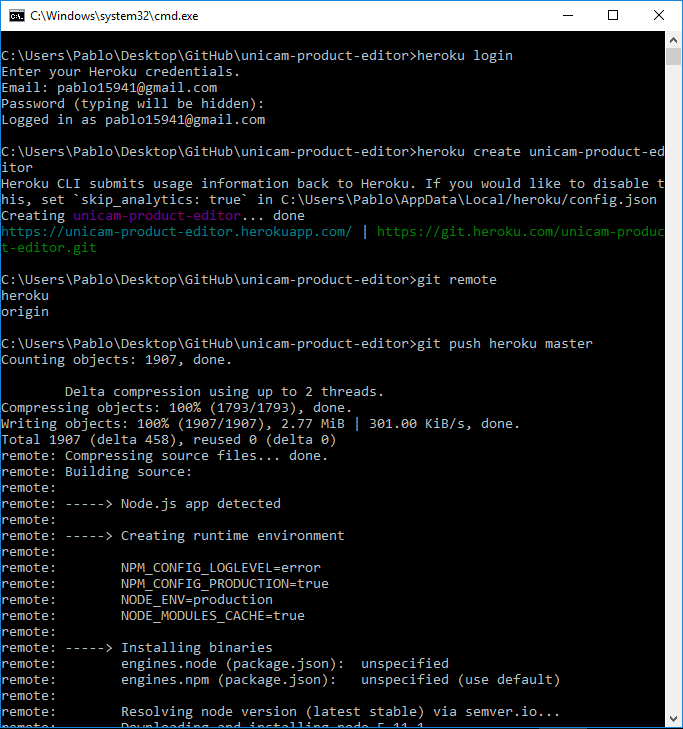
\includegraphics[scale=0.7]{Immagini/heroku_initialize.png}
	\caption{Inizializzazione di unicam-product-editor su Heroku}
\end{figure}
\begin{figure}[h]
	\centering
	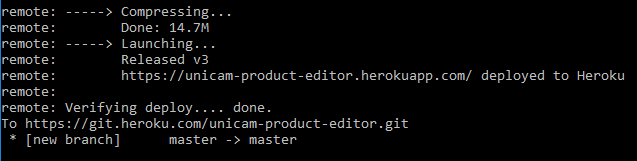
\includegraphics[scale=0.8]{Immagini/heroku_deployment.png}
	\caption{Rilascio di unicam-product-editor su Heroku}
\end{figure}
\chapter{Long Polling}
\label{chap:long_polling}
In questo capitolo si spiega il funzionamento del modello di comunicazione 
Long Polling, per poi spiegare come è applicato in unicam-product-editor, 
ed infine compararlo con altre metologie in uso.

L'XMLHTTPRequest Long Polling è, di base, una tecnologia dove il client 
richiede un'informazione al server senza aspettarsi una risposta immediata.
Questo fa sì che la connessione che esiste fra client e server abbia una 
connessione di lunga durata, durante la quale il server esegue un'operazione 
complessa, e solo una volta portata a termine, restituisce una risposta al 
client inviando i dati richiesti come risposta, o anche solo una notifica.

Innanzitutto il fatto che questa tecnologia sia basata su XMLHTTPRequest 
ci fa capire che le chiamate che il client effettua nei confronti del 
server sono delle semplici chiamate Ajax, ma a differenza dell'uso 
tradizionale di queste chiamate, la gestione degli eventi non viene 
eseguita dalla parte del client (client-side), ma dalla parte del 
server (server-side).Inoltre, a differenza delle chiamate Ajax, che 
vengono effettuate a intervalli regolari, ad esempio ogni 10 secondi 
al termine delle quali la connessione al server viene chiusa, in una 
chiamata di tipo Long Polling, la connessione col server rimane aperta 
finché il server stesso non invia una risposta, oppure finché non si 
raggiunge un limite di tempo impostato, detto timeout.

Questo tipo di tecnlogia usato nelle applicazioni non è nuovo, le web 
chat sono sempre esistite. Quello che è cambiato negli ultimi anni è 
l’approccio tecnologico a basso livello. Una volta i client facevano 
richieste HTTP ogni pochi secondi al server richiedendo eventuali 
messaggi (come ad esempio nel protocollo POP3 per la ricezione delle 
email) mentre nel Long Polling è il server stesso a notificare il 
client solamente a fronte di novità.
\newpage
Di seguito uno schema che riassume l'architettura Long Polling, 
mostrando l'interazione fra un client e un server, e le relative 
richieste e risposte.
\begin{figure}[h]
	\centering
	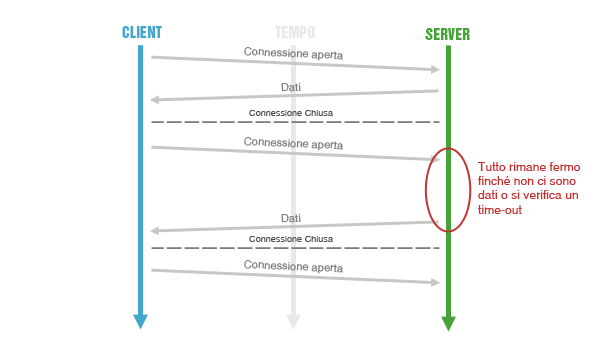
\includegraphics[scale=0.7]{Immagini/long_polling.png}
	\caption{Modello di comunicazione Long Polling}
\end{figure}

Questo metodo, assieme ad altri con lo stesso funzionamento di base 
(ad esempio lo Streaming) insieme costituiscono il modello architetturale 
Comet, in cui le richieste HTTP di lunga durata che permettono ad un web 
server di inviare dati ad un browser senza che quest'ultimo li abbia 
esplicitamente richiesti ne sono la caratteristica principale.

La tecnica del Long Polling, nonostante non sia difficilissima da 
implementare una volta compresa, non può essere però eseguita in 
qualsiasi server web proprio per la caratteristica di avere richieste 
in stato “pending”. I principali server web e application server non 
offrono questa funzionalità nativa perchè agiscono, differentemente da 
Node.js, in maniera sincrona. Hanno a disposizione un numero finito di 
“slot di richieste”, esaurito il quale sono obbligati a rilasciarne qualcuna.
NodeJS grazie al suo modello \emph{event-driven} offre una struttura di 
basso livello che eccelle in questo tipo di applicazioni. Il meccanismo 
basato su callback rappresenta il deux ex machina per un architettura 
basata su Long Polling.

In unicam-product-editor, e più precisamente nella fase di upload di 
un oggetto 3D, il caso base che si verificherà sarà quello del client 
che inizia il caricamento della forma attraverso l'interfaccia, 
inviando una richiesta HTTP al server Node.js, il quale inizierà in 
sequenza le fasi di upload, conversione in JSON e inserimento del file 
convertito nel database. Durante questo processo, che per sua natura 
ha un tempo di esecuzione lungo (essendo i file 3D in formato .obj ed 
i corrispondenti file JSON una dimensione media nell'ordine dei MegaByte) 
la richiesta HTTP rimane in una fase di congelamento, finché il server 
non avrà eseguito tutto il processo, ed invierà al client una risposta 
(sia essa di successo nell'esecuzione o di errore), o finché non si 
sarà raggiunto il tempo limite, detto timeout, superato il quale la 
richiesta si esaurirà.

Il Long Polling HTTP inoltre è utilissimo per creare API affidabili, 
in quanto le azioni di sincronizzazione e di ascolto possono essere 
combinate in una stessa richiesta. Nel nostro caso, essendo questo 
progetto basato su RESTful API, è facile espandere una di queste 
trasformandola in una Long Polling API, mantenendo comunque la stessa 
semantica, usando anche questo sistema delle interazioni di tipo 
\emph{request/response}. Dei timeout brevi possono oltretutto aumentare 
la solidità delle richieste fra client e server nel caso in cui, ad 
esempio, l'indirizzo IP di un client cambi come conseguenza del roaming 
da rete wireless a rete mobile o tethering.

E' per questi motivi che in unicam-product-editor è stata implementata 
la tecnologia di Long Polling nella fase di upload di una forma 3D.
Il tutto rende il processo di upload non bloccante, ossia permette 
all'utente, durante l'esecuzione delle operazioni sopra elencate, di 
continuare ad eseguire altre operazioni sulla applicazione web, mentre 
il processo viene portato a termine in background.
Per rendere ciò possibile, dobbiamo ricordarci che il progetto è basato 
su un server Node.js, il quale è di tipo \emph{event-driven}, ed esegue 
le operazioni in modo asincrono. Proprio per questa caratteristica, 
la fase di upload di un oggetto 3D non è bloccante nei confronti 
dell'utente, che può così continuare ad inviare al server normali 
richieste HTTP.

\section{Implementazione del Long Polling in unicam-product-editor}
In questa fase andremo a vedere l'uso pratico della tecnologia appena 
descritta nel nostro editor di forme 3D.

Per quanto riguarda le normali chiamate HTTP Ajax, è stata usata 
jQuery\cite{jquery}, una libreria JavaScript veloce, leggera e 
ricca di funzionalità.

Prendiamo in esame il Controller Angular su cui si sviluppa la 
pagina dell'uploader:

\begin{lstlisting}[{caption=HTTP POST /upload}, style=JavaScriptCode]
$http.post('/upload', fd, {
	withCredentials: true,
	headers: {'Content-Type': undefined },
	transformRequest: angular.identity
})
\end{lstlisting}
Per prima cosa si esegue la HTTP POST request relativa all'upload e 
successiva conversione del file .obj. La chiamata API è indicata 
subito dopo la funzione \texttt{\$http.post}, ed è \texttt{/upload}.
La risposta che arriverà da parte del server sarà l'endpoint del 
file JSON convertito, che metteremo nella variabile \texttt{filename}.
Dopo questo si esegue una chiamata HTTP GET, passando come parametro 
il nome del file appena convertito, per inserire il file JSON nel database.  

\begin{lstlisting}[{caption=HTTP GET /insert}, style=JavaScriptCode]
$http({method: 'GET', url: filename})
	.then(function successGet(filename) {
		$http({method: 'POST',
			url: '/insert',
			data: {shape: filename.data}
		})
	...
\end{lstlisting}

La gestione degli errori avviene tramite la funzione \texttt{.then} 
della richiesta HTTP: se l'operazione va a buon fine, la risposta 
del server sarà il codice \texttt{200, OK}, mentre in caso 
contrario il server risponderà con un codice di errore. In entrambi 
i casi il risultato è contenuto nel parametro \texttt{response}.

\begin{lstlisting}[{caption=gestione degli errori nella richiesta HTTP}, style=JavaScriptCode]
.then(function successResponse(response){
	console.log(response);
	console.log('file inserted in db');
	$scope.isRouteLoading = false;
	$scope.uploadsuccess = true;
}, function errorResponse(response) {
	console.log(response);
	console.log('error in insert');
});
\end{lstlisting}

\section{Altri metodi di comunicazione fra client e server}
Di seguito vengono elencati, oltre al Long Polling, gli altri 
metodi di comunicazione fra client e server, con particolare 
riguardo al modo in cui vengono scambiate le richieste fra i 
due interlocutori.

\subsection{Normale HTTP}
\begin{enumerate}
	\item Il client richiede una pagina web al server.
	\item Il server calcola la risposta.
	\item Il server invia la risposta al client.
\end{enumerate}
\begin{figure}[h]
	\centering
	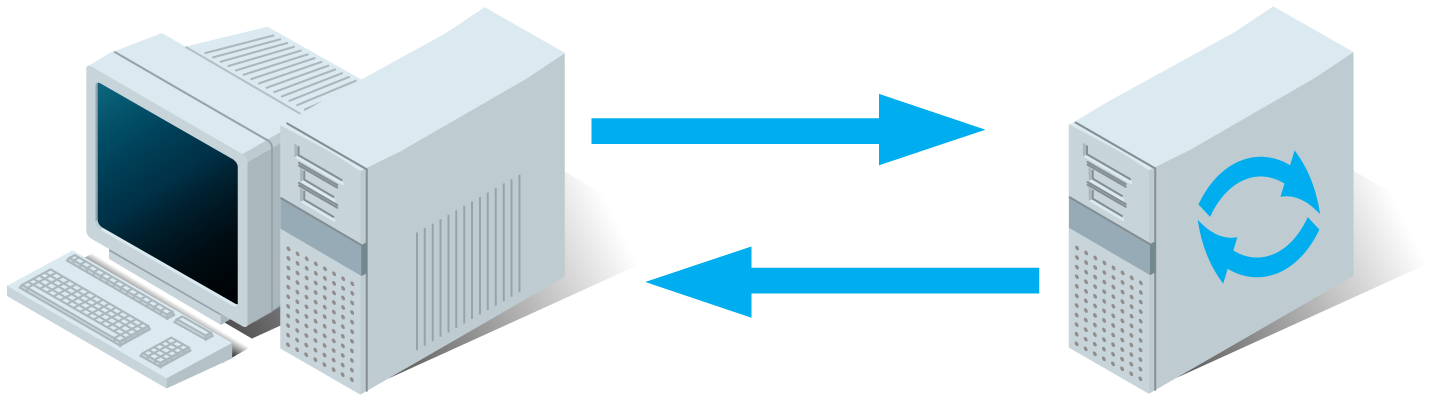
\includegraphics[scale=0.4]{Immagini/regular_http.png}
\end{figure}
\subsection{Polling Ajax}
\begin{enumerate}
	\item Il client richiede una pagina web al server usando  il normale HTTP.
	\item Il client riceve la pagina web richiesta ed esegue il codice JavaScript contenuto nella pagina, il quale richiede un file al server ad intervalli regolari (es. 0.5 secondi).
	\item Il server calcola ogni risposta e la invia al client, come del normale traffico HTTP.
\end{enumerate}
\begin{figure}[h]
	\centering
	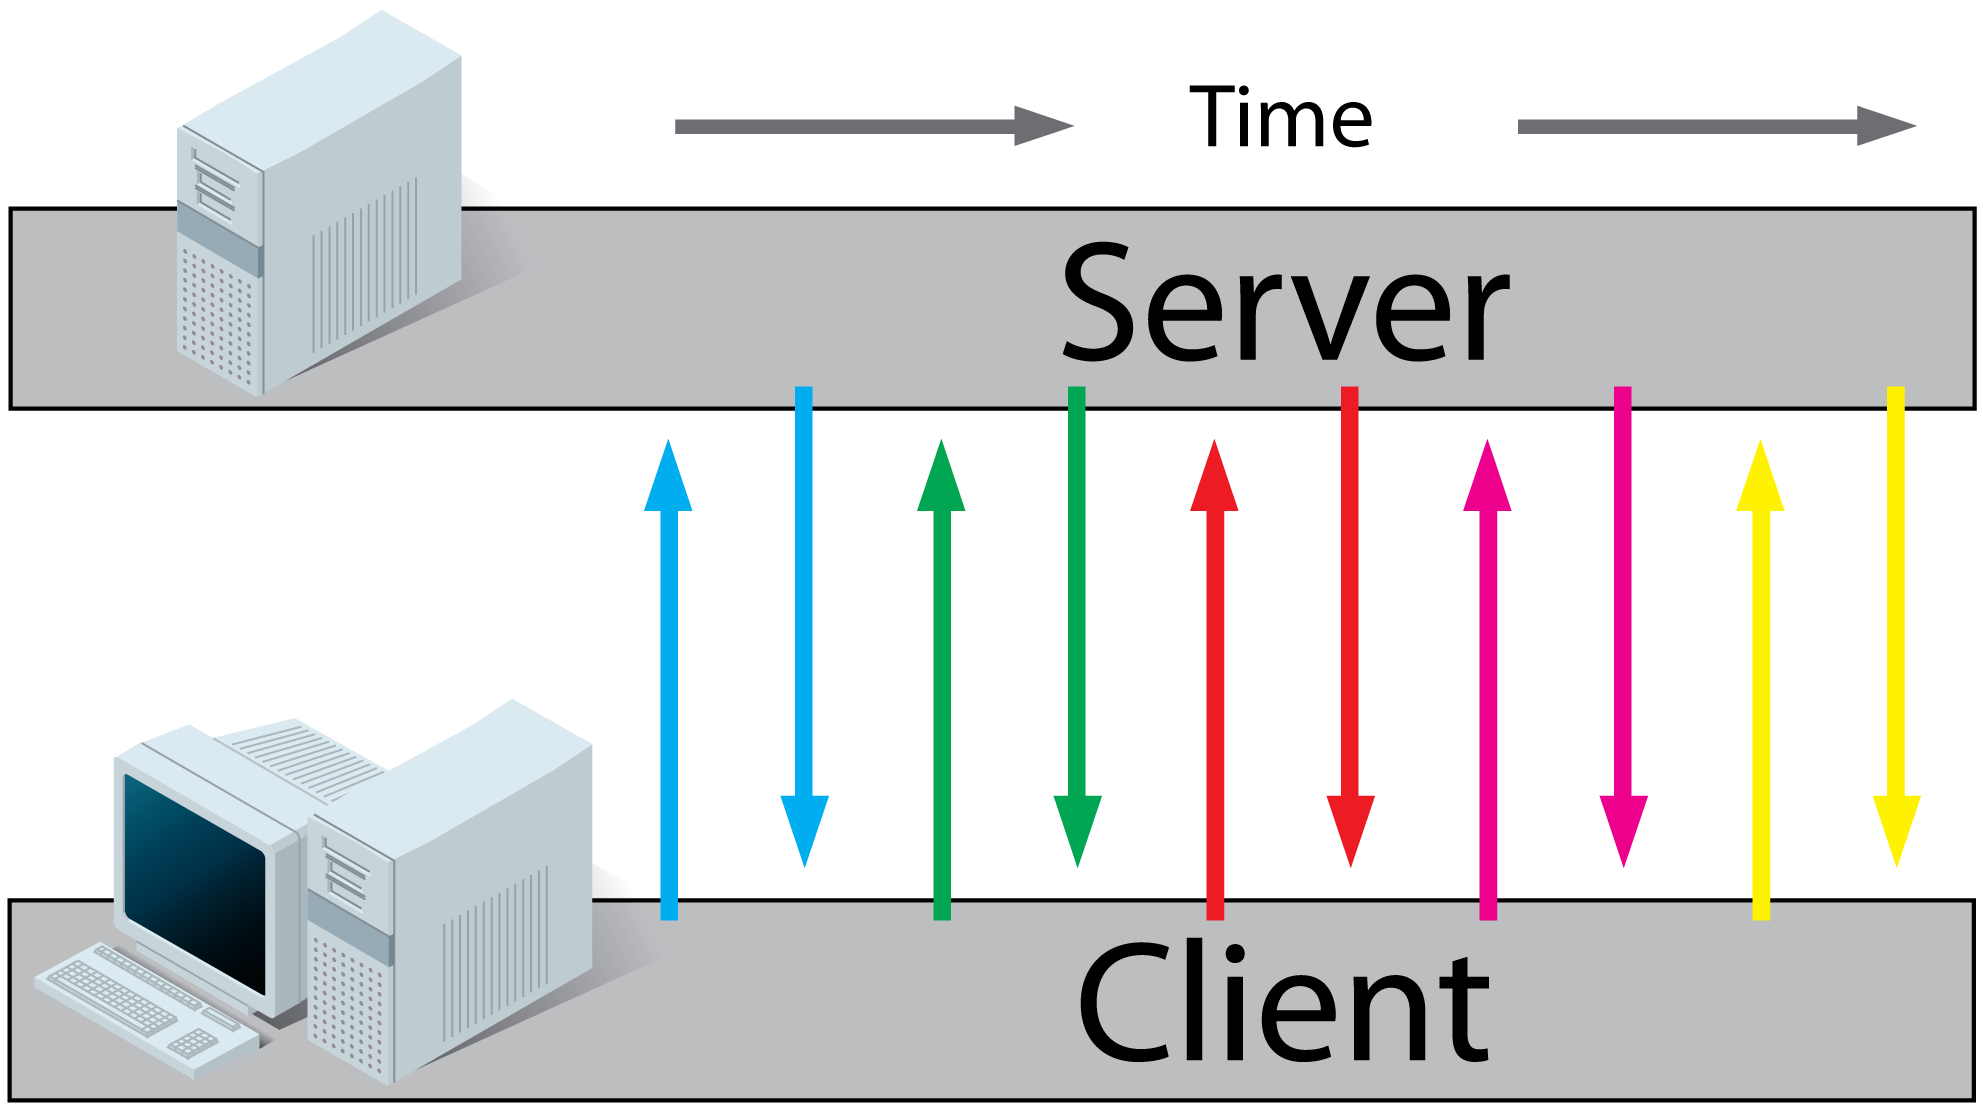
\includegraphics[scale=0.4]{Immagini/ajax_polling.png}
\end{figure}
\subsection{Long Polling Ajax}
\begin{enumerate}
	\item Il client richiede una pagina web al server usando il normale HTTP.
	\item Il client riceve la pagina web richiesta ed esegue il codice JavaScript contenuto nella pagina, il quale richiede un file al server.
	\item Il server non risponde immediatamente con l'informazione richiesta, ma aspetta finché non c'è una nuova informazione disponibile.
	\item Quando l'informazione è disponibile, il server risponde con questa.
	\item Il client riceve la nuova informazione e manda immediatamente un'altra richiesta al server, riavviando il processo.
\end{enumerate}
\begin{figure}[h]
	\centering
	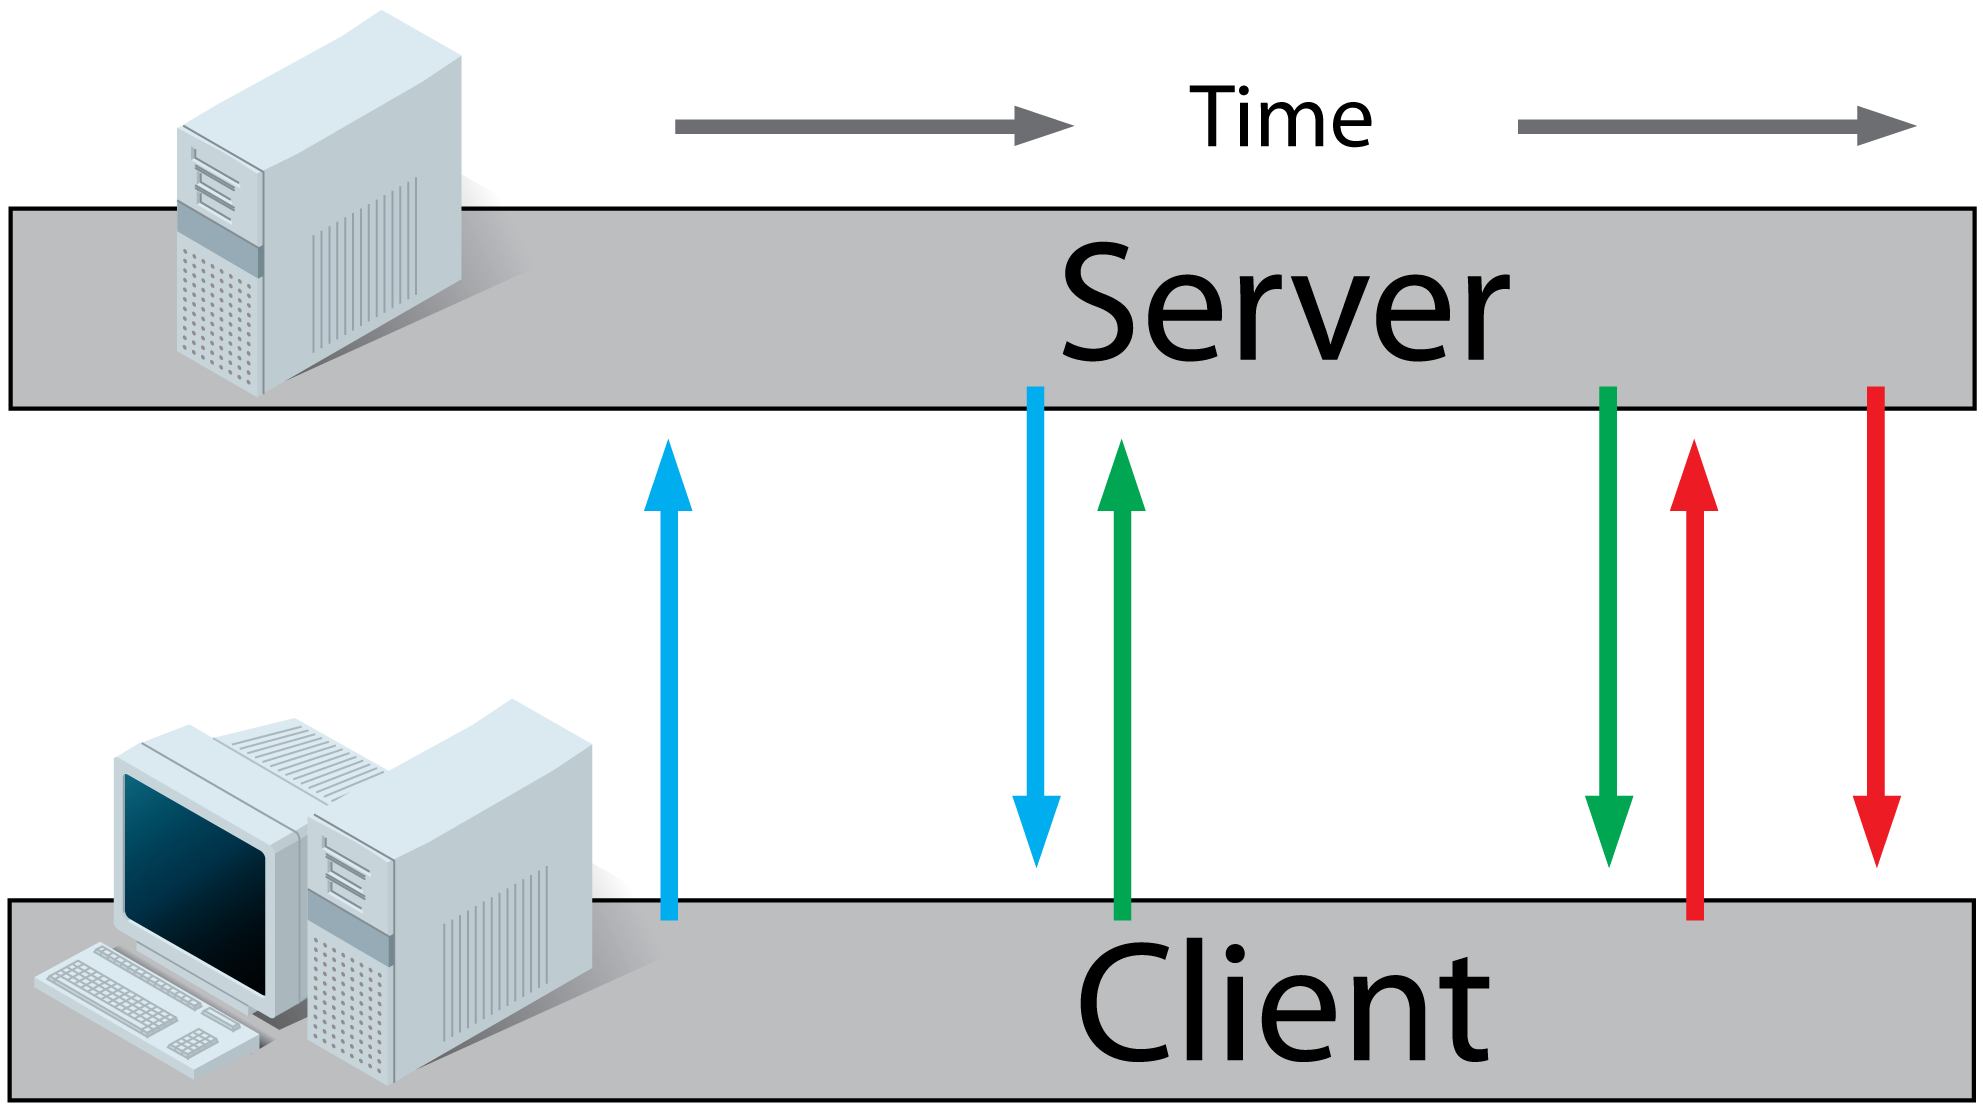
\includegraphics[scale=0.4]{Immagini/ajax_long_polling.png}
\end{figure}
\subsection{HTML5 Server Sent Events (SSE)}
\begin{enumerate}
	\item Il client richiede una pagina web al server usando il normale HTTP.
	\item Il client riceve la pagina web richiesta ed esegue il codice JavaScript contenuto nella pagina, il quale apre una connessione al server.
	\item Il server invia un evento al client non appena è disponibile una nuova informazione.
\end{enumerate}
\begin{figure}[h]
	\centering
	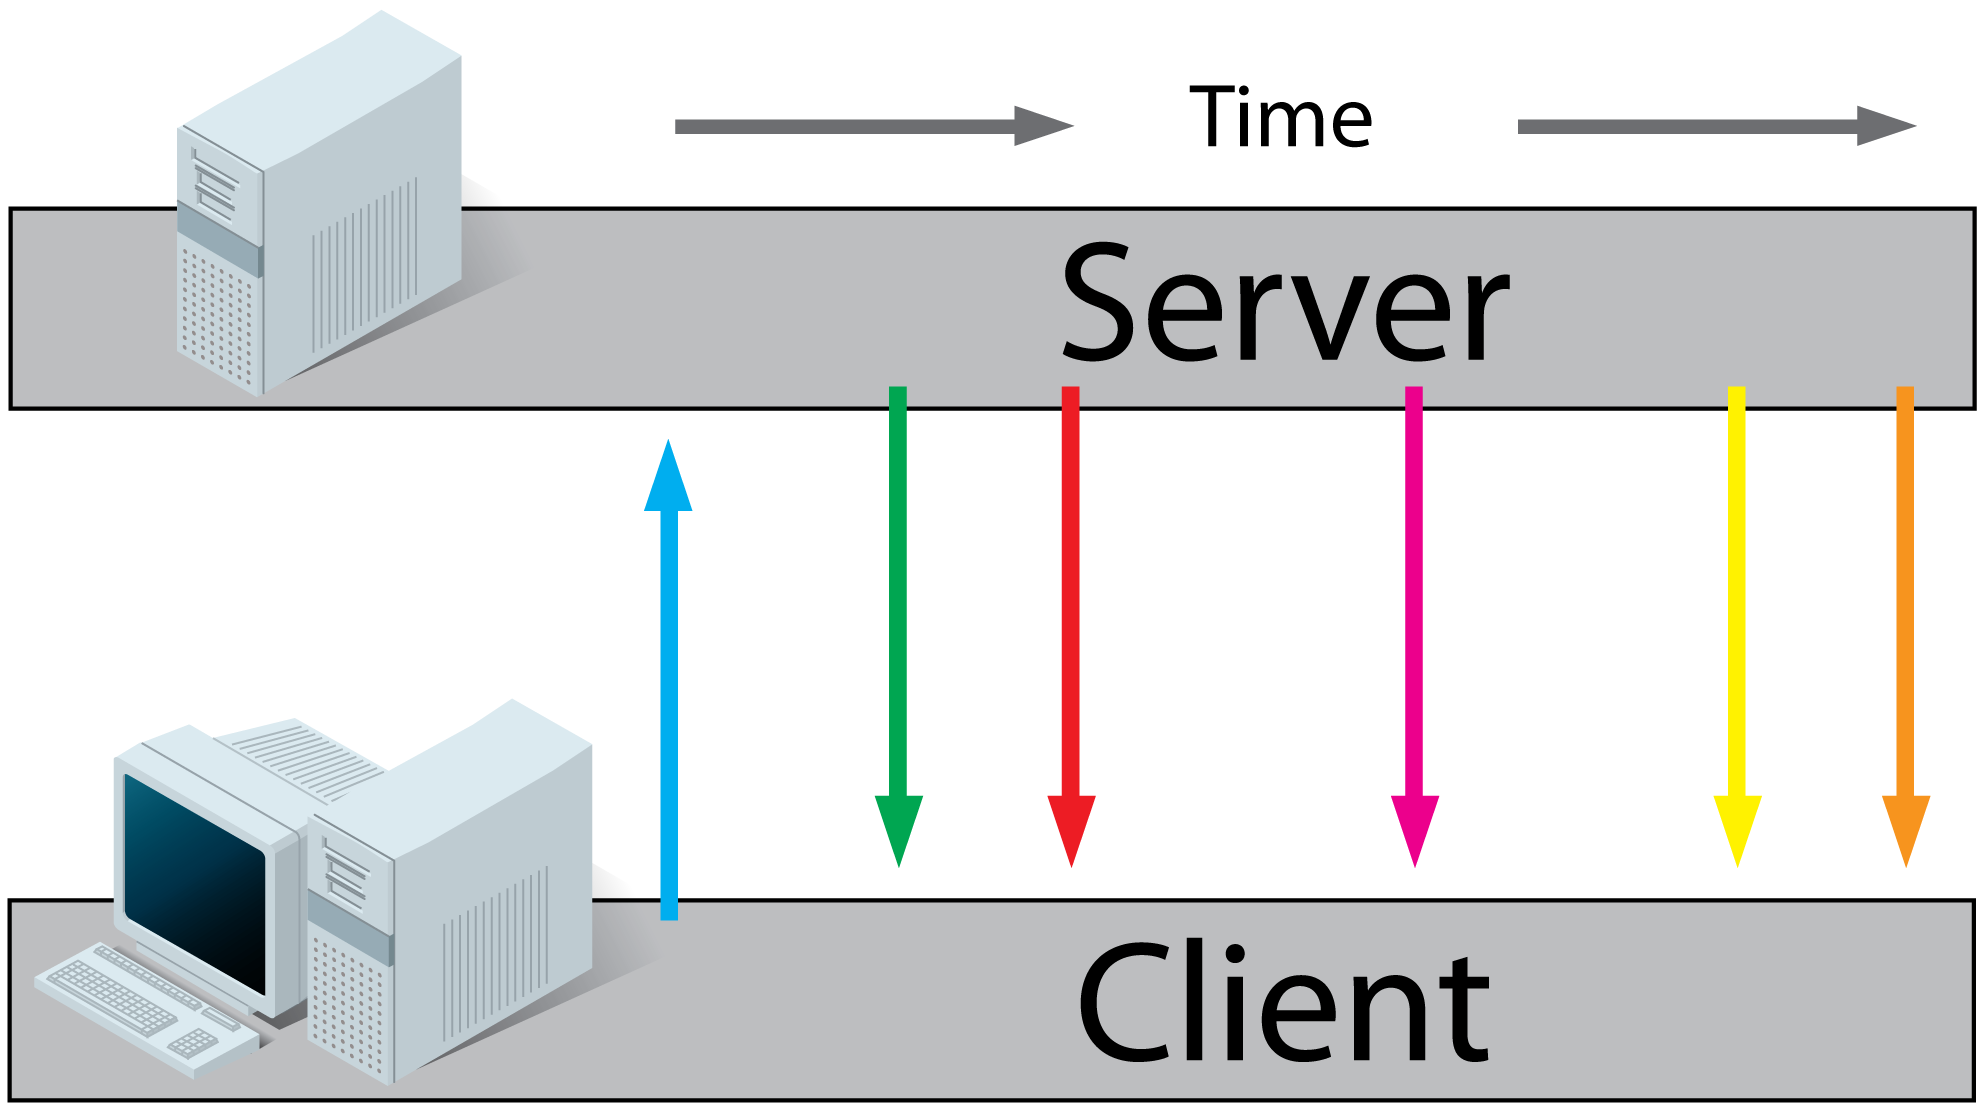
\includegraphics[scale=0.4]{Immagini/server_sent_events.png}
\end{figure}
\newpage
\subsection{HTML5 Websockets}
\begin{enumerate}
	\item Il client richiede una pagina web al server usando il normale HTTP.
	\item Il client riceve la pagina web richiesta ed esegue il codice JavaScript contenuto nella pagina, il quale apre una connessione al server.
	\item Il client e il server possono ora scambiarsi messaggi quando sono disponibili nuove informazioni (da qualsiasi lato).
\end{enumerate}
\begin{figure}[h]
	\centering
	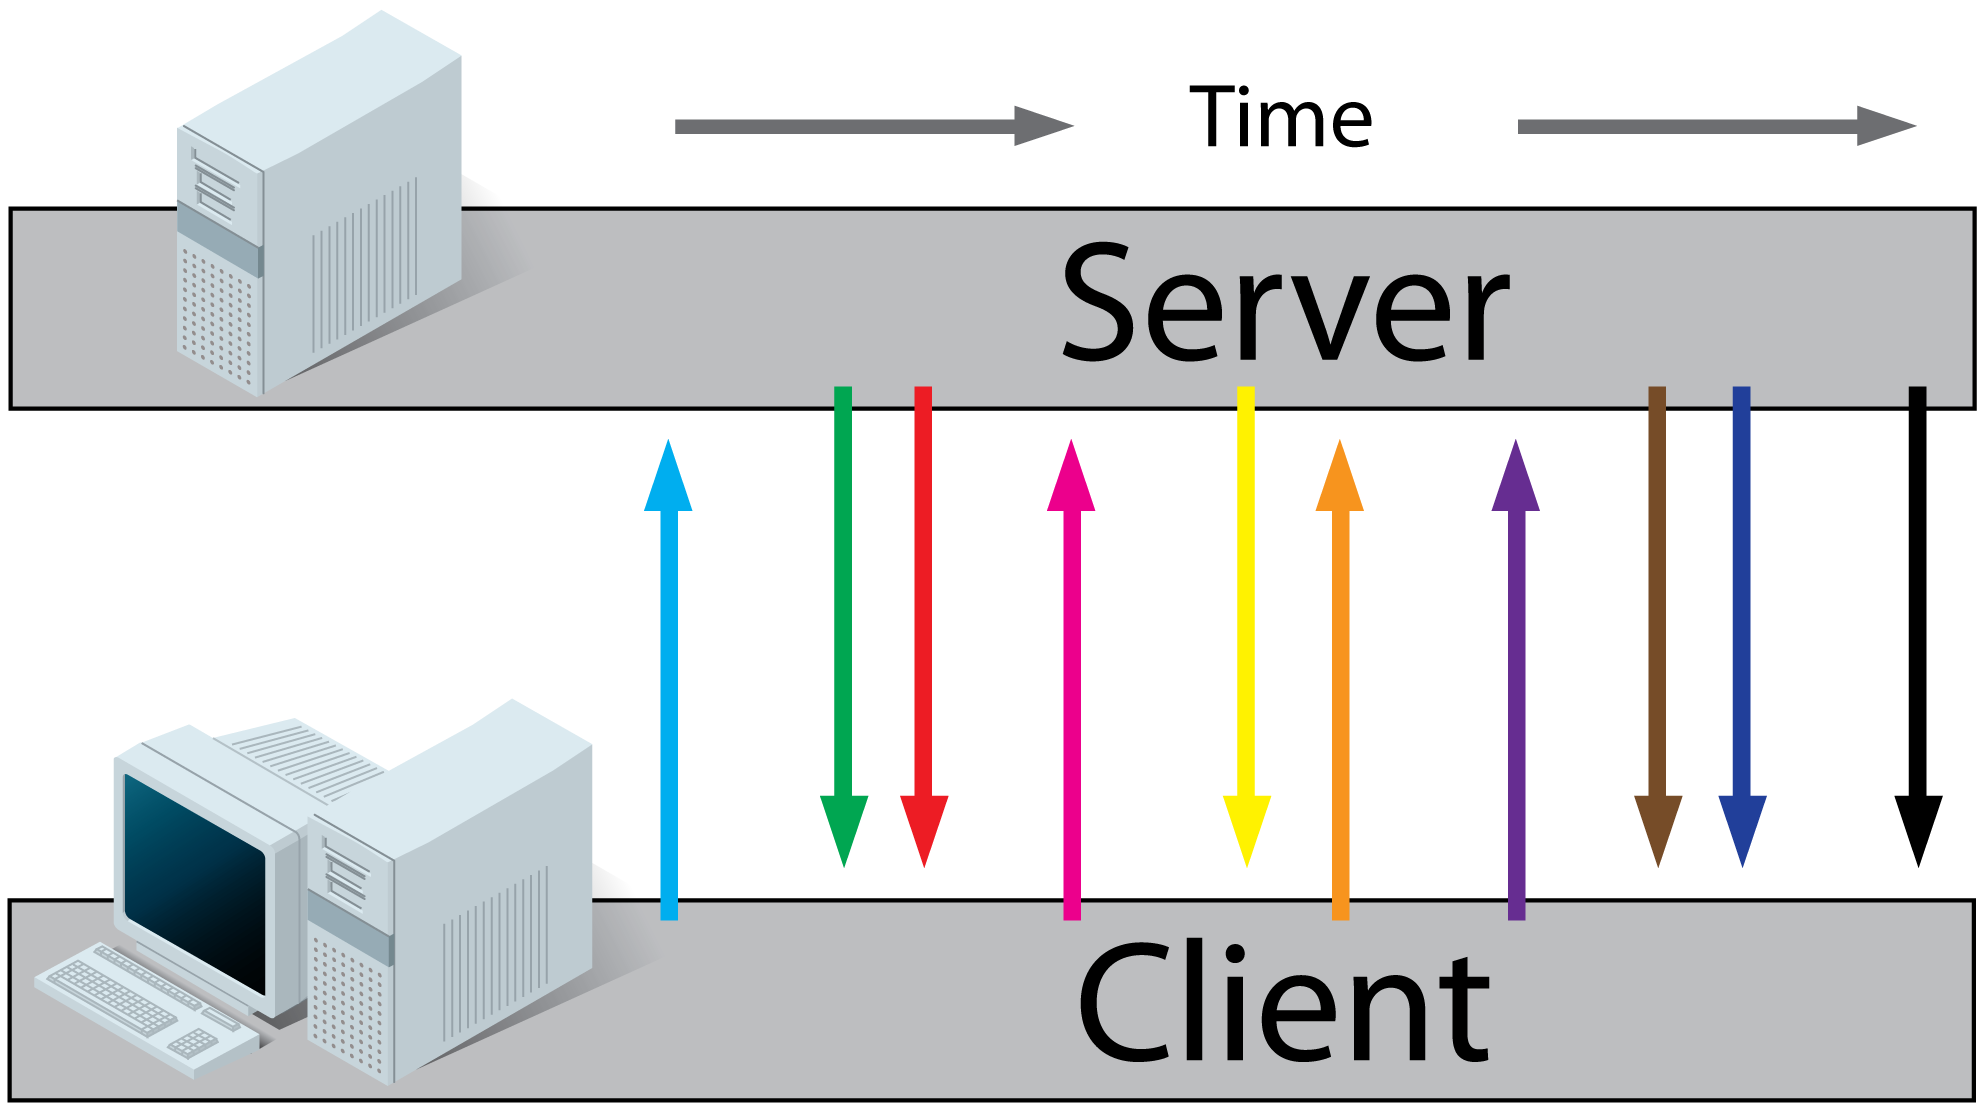
\includegraphics[scale=0.4]{Immagini/websockets.png}
\end{figure}
\chapter{Implementazione}
\label{chap:implementazione}
In questo capitolo si mostra come sono state implementate le funzionalità richieste dalle user stories mostrate nella tabella \ref{tab:user:sto}.
Per ogni funzionalità vedremo quali API sono state create, come sono state documentate attraverso Postman ed il codice utilizzato per realizzarle.

Tutte le rotte relative ai servizi API sono presenti nel file \texttt{/routes.js}, ad esclusione dei servizi relativi alla registrazione e autenticazione di un utente, che si trovano direttamente nel file \texttt{/app.js}.
\section{US-01/03}
Per l'implementazione delle prime tre user stories, che verrano trattate insieme, essendo per lo più simili tra loro, sono stati creati i seguenti servizi:
\begin{lstlisting}[{caption=/routes.js}, style=JavaScriptCode]
module.exports = function(app){
	var List = require('./controllers/lists');
	var Object = require('./controllers/objects');
	var Part = require('./controllers/parts');
	var Option = require('./controllers/options');
	
	app.get('/lists', List.findAll);
	app.get('/lists/:id', List.findById);
	app.post('/lists', List.add);
	app.put('/lists/:id', List.update);
	app.delete('/lists/:id', List.delete);
	
	app.get('/objects/:listid', Object.findAll);
	app.get('/objects/:id', Object.findById);
	app.post('/objects/:listid', Object.add);
	app.put('/objects/:id', Object.update);
	app.delete('/objects/:id', Object.delete);
	
	app.get('/parts/:objectid', Part.findAll);
	app.get('/parts/:id', Part.findById);
	app.post('/parts/:objectid', Part.add);
	app.put('/parts/:id', Part.update);
	app.delete('/parts/:id', Part.delete);
	
	app.get('/options/:partid', Option.findAll);
	app.get('/options/:id', Option.findById);
	app.post('/options/:partid', Option.add);
	app.put('/options/:id', Option.update);
	app.delete('/options/:id', Option.delete);
}
\end{lstlisting}
Come si può vedere, ad ogni operazione CRUD è associata la relativa API, che esegue una specifica funzione presente nel file corrispondente. I file relativi alle suddette funzioni sono contenuti nella cartella \texttt{controllers} e vengono richiamati all'inizio del file \texttt{routes.js}.

Le funzioni sono sufficientemente autoesplicative, ma per chiarezza vengono elencate ed esposte qui di seguito:
\begin{itemize}
	\item \texttt{app.get} si divide in due casi:
	\begin{enumerate}
		\item \texttt{/API} in cui vengono richiesti tutti i Document di una Collection. Nel caso in cui la Collection sia un Object, una Option o una Part, viene passato in input il parametro \texttt{:id} che identifica il Document \emph{parente}.
		\item \texttt{/API/:id} in cui viene passato il parametro \texttt{:id}, per interrogare la Collection nel database MongoDB secondo il criterio di identificazione.
	\end{enumerate}
	\item \texttt{app.post} \\Con questa operazione si aggiunge un Document alla corrispondente Collection. Questo è l'unico caso in cui vanno distinte le Lists dagli altri oggetti. Quando si aggiunge una List tramite metodo POST, non viene passato nessun parametro alla chiamata API. Si noti invece che negli altri casi, durante la medesima operazione, viene sempre passato l'id dell'oggetto \emph{parente}, dell'oggetto ossia a cui fa riferimento il Document che stiamo inserendo.
	\item \texttt{app.put} \\Questa operazione viene usata per modificare un Document già presente in una Collection. Prende in input il parametro \texttt{:id} per poter ritrovare il giusto oggetto su cui eseguire un \emph{update}.
	\item \texttt{app.delete} \\Infine l'operazione \emph{delete} si usa per eliminare un Document specifico, che viene identificato, come sopra, prendendo in input il parametro \texttt{:id}. 
\end{itemize}

Di seguito prendiamo in esame il controller relativo agli Objects per analizzare le relative funzioni, seguite dalla relativa documentazione realizzata con Postman:
\begin{lstlisting}[{caption=/controllers/objects.js}, style=JavaScriptCode]
var mongoose = require('mongoose'),
Object = require('../app/schema.js').model('Object');

exports.findAll = function(req, res){
	var listid = req.params.listid;
	Object.find({'_list': listid},function(err, docs) {
		return res.send(docs);
	});
};

exports.findById = function(req, res){
	var id = req.params.id;
	Object.findOne({'_id': id, '_list': listid},function(err, docs) {
		return res.send(docs);
	});
};

exports.add = function(req, res) {
	var listid = req.params.listid;
	Object.create({"nome": req.body.nome, "descrizione": req.body.descrizione, 
	"_list": listid}, function (err, docs) {
		if (err) return console.log(err);
		return res.send(docs);
	});
};

exports.update = function(req, res) {
	var id = req.params.id;
	var updates = req.body;
	console.log(id);
	Object.update({"_id":id}, req.body,
	function (err, numberAffected) {
		if (err) return console.log(err);
		console.log('Updated %d Lists', numberAffected);
		return res.sendStatus(202);
	});
};

exports.delete = function(req, res) {
	var id = req.params.id;
	Object.remove({'_id':id},function(result) {
		return res.send(result);
	});
};
\end{lstlisting}

L'interfacciamento con il database è gestito tramite mongoose, di cui viene importata la dipendenza all'inizio del file.
La prima funzione è \texttt{findAll}, che prende in input, attraverso i parametri presenti nella request, l'id della List a cui l'Object è associato. Viene quindi eseguita la funzione \texttt{.find} di mongoose sulla Collection Objects, filtrando per l'id appena passato, e quello che si avrà come risposta sarà una callback, che conterrà un messaggio di errore in caso di fallimento, o i Document richiesti in caso di successo. A questo punto il server invia la risposta tramite la funzione \texttt{res.send}, includendo i risultati dell'interrogazione appena effettuata sul database. La funzione \texttt{findById} è molto simile alla precedente, pertanto non verrà spiegata nuovamente.
\begin{figure}[h]
	\centering
	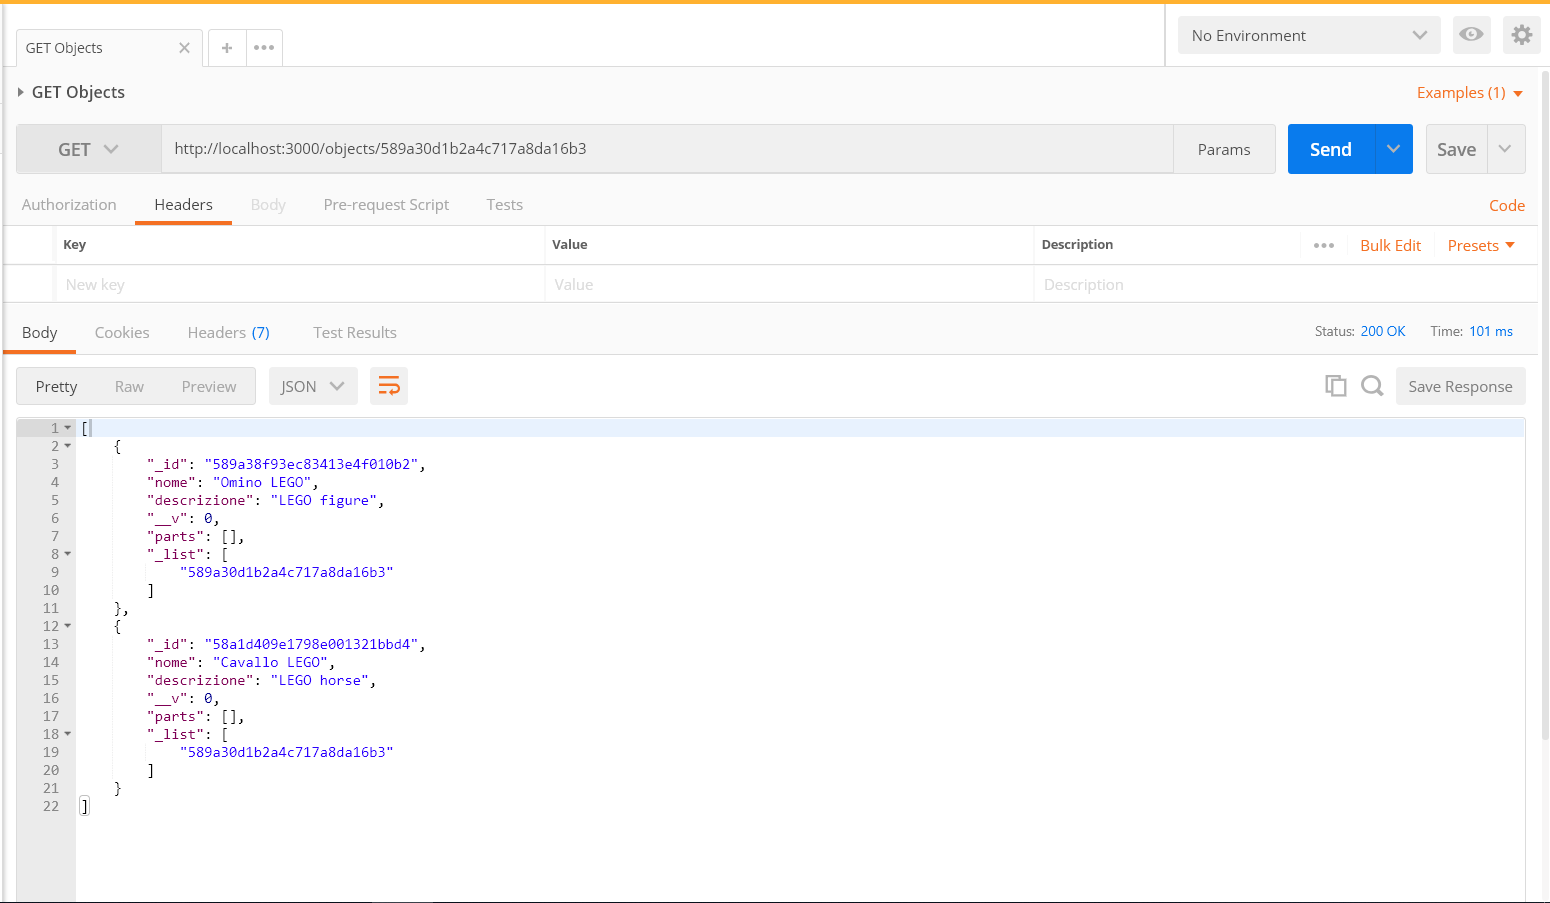
\includegraphics[scale=0.42]{Immagini/get_objects.png}
	\caption{Documentazione get /objects/:id}
\end{figure}

La funzione \texttt{add} inserisce un nuovo Object Document nella sua Collection, solo dopo però averlo inizializzato inserendo l'id della List a cui fa riferimento nell'attributo \texttt{\_list}, il nome (preso dal \emph{body} della richiesta HTTP) nell'attributo \texttt{nome} e la descrizione nel corrispondente attributo. I parametri nome e descrizione sono stati inseriti dall'utente negli appositi campi presenti nella pagina di visualizzazione degli Objects, e vengono trasmessi al server attraverso la richiesta HTTP POST.
\begin{figure}[h]
	\centering
	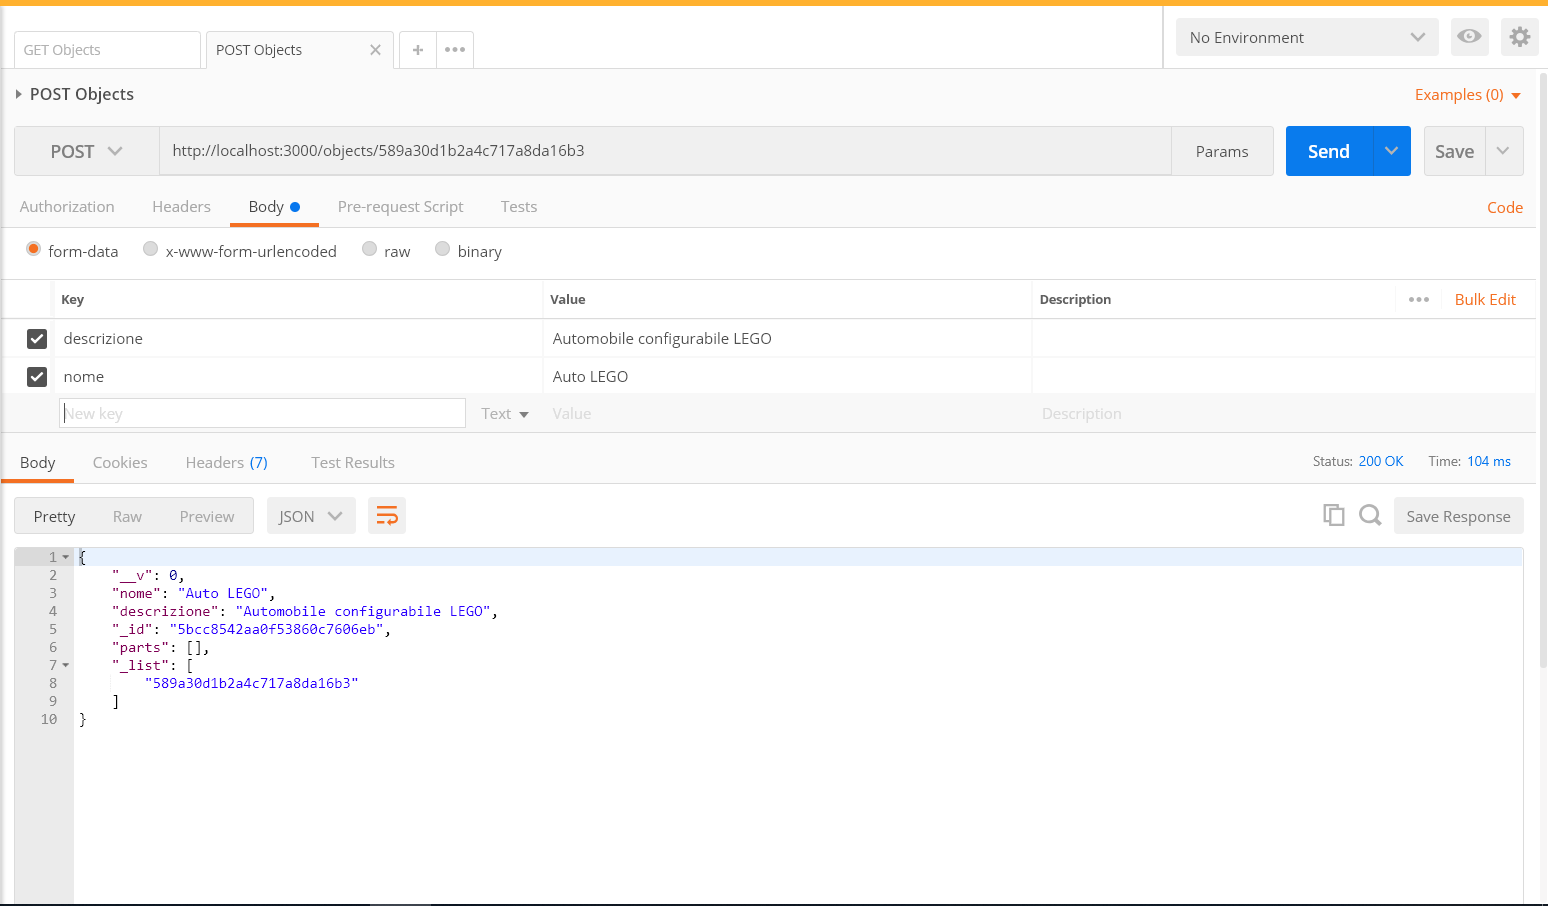
\includegraphics[scale=0.42]{Immagini/post_objects.png}
	\caption{Documentazione post /objects/:id}
\end{figure}

L'ultima funzione è \texttt{delete}. Questa rimuove l'Object cercandolo attraverso il suo \texttt{id}. La funzione non necessita di alcun parametro aggiuntivo.
\begin{figure}[h]
	\centering
	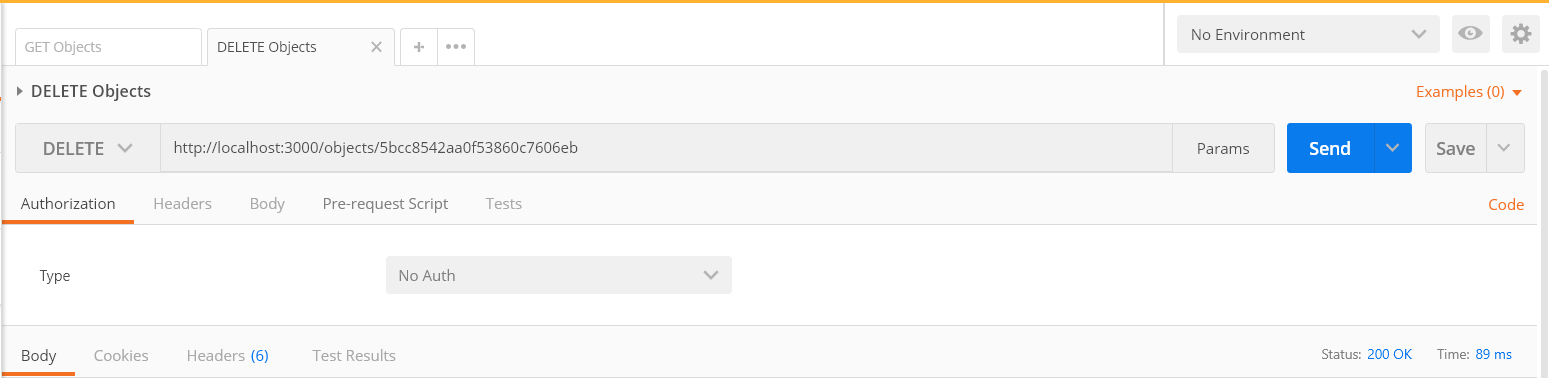
\includegraphics[scale=0.42]{Immagini/delete_objects.png}
	\caption{Documentazione delete /objects/:id}
\end{figure}

Le funzioni si comportano in modo analogo, o comunque come spiegato sopra, con gli altri tipi di oggetti in unicam-product-editor.
Per quanto riguarda la funzione di visualizzazione dei documenti richiesta dalle user stories dalla 01 alla 03, è stata sviluppata una applicazione single-page in AngularJS, che andremo a vedere nella US-05.
\section{US-04}
La user story 04 richiede di avere un endpoint che restituisca la forma JSON di un oggetto 3D da visualizzare.

Per implementare questa funzione, è stata creata una chiamata API apposita, contenuta nel file del server \texttt{app.js}.

\begin{lstlisting}[{caption=shape API}, style=JavaScriptCode]
app.get('/shape/:id', cors(corsOptions), function(req, res){
	var search = req.params.id;
	converted(req, search, res);
});
\end{lstlisting}
Come possiamo vedere dallo snippet di codice qui sopra, la API rimanda alla apposita funzione converted, situata in \texttt{/app/converted.js}.

\begin{lstlisting}[{caption=/app/converted.js}, style=JavaScriptCode]
coll.find({"_id" : mongodb.ObjectId(search)}).toArray(function(err, docs) {
	if (err){
		console.log('error in db');
		res.end();
		return;
	}
	else if (docs.length == '0'){
		console.log('No files found');
		res.send('No files found');
	}
	else{
		res.send(docs);
	}
});
\end{lstlisting}
Lo scopo della funzione è quello di trovare nella Collection Shapes il documento JSON corrispondente a quello dell'id richiesto. In questa particolare Collection, i JSON non seguono uno Schema come nel caso degli altri oggetti, ma vengono conservati così come sono, essendo questi il risultato della conversione dei file .obj. Così quando il server risponderà, non lo farà usando uno stato risultante di una richiesta HTTP, ma lo farà inviando il JSON vero e proprio. Grazie a questo tipo di risposta, unicam-product-viewer avrà il suo enpoint a cui agganciarsi per prendere le forme 3D da visualizzare nella propria interfaccia.
\begin{figure}[h]
	\centering
	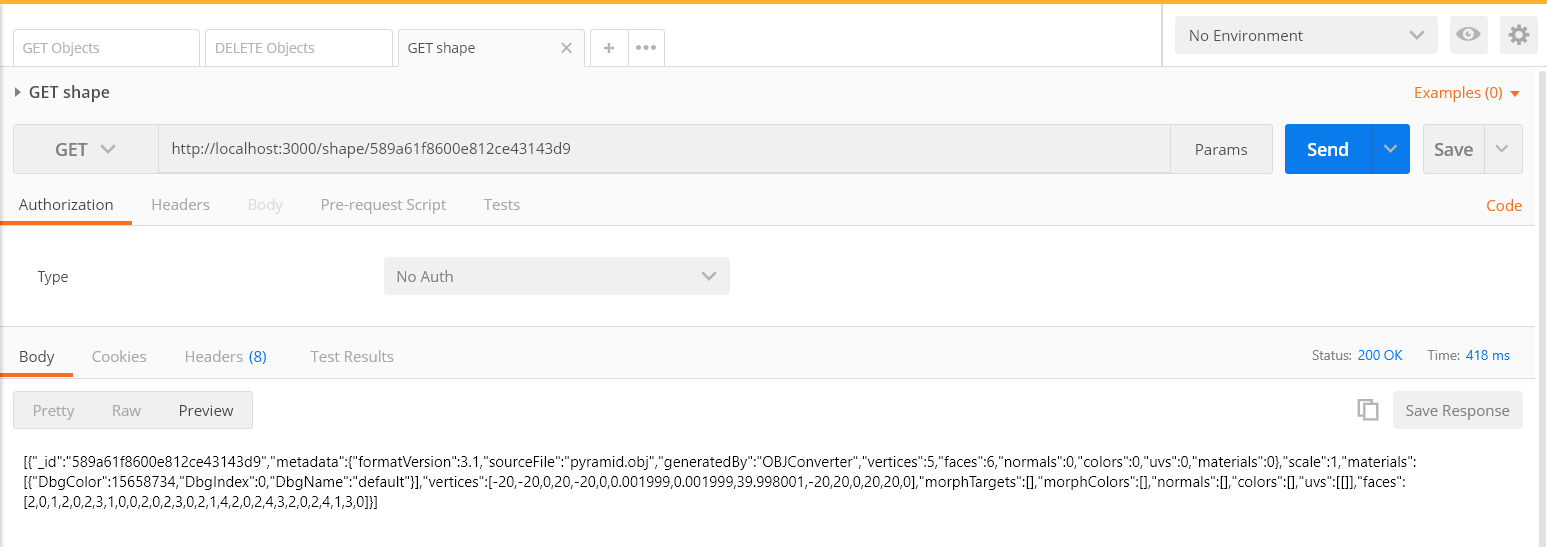
\includegraphics[scale=0.42]{Immagini/get_shape.png}
	\caption{Documentazione get /shape/:id}
\end{figure}

\chapter{Conclusioni}
\label{chap:conclusioni}
Lo scopo di questa tesi era quella di sviluppare un editor di oggetti 3D configurabile, 
e che usasse la realtà aumentata.Con gli argomenti trattati abbiamo visto come negli 
ultimi anni la tendenza sia quella di usare il linguaggio JavaScript non per l'esecuzione 
di pochi controlli nelle pagine web come veniva fatto nei primi anni successivi alla 
sua nascita, ma come un linguaggio di riferimento per lo sviluppo di applicazioni 
sia lato client che lato server. JavaScript è ormai usato per sistemi distribuiti, 
ed eseguibili su qualsiasi dispositivo che lo supporti, indipendentemente da sistema 
operativo e hardware utilizzati.Abbiamo visto l'utilizzo di database documentali al 
posto dei database relazionali, evidenziandone le principali differenze.Il frutto 
dell'utilizzo di queste tecnologie combinate è una applicazione web eseguibile 
attraverso un semplice browser, ma con caratteristiche e prestazioni quasi o del 
tutto equiparabili ad un'applicazione desktop tradizionale.

La tecnologia sviluppata con questo progetto, data dall'insieme di unicam-product-editor
 e unicam-product-viewer apre le porte ad un nuovo modo di interpretare la visualizzazione
  dei prodotti nell'e-commerce, che fino ad oggi si è basata su tecnologie semplici 
  ed efficaci, ma che nel corso degli anni non hanno mai avuto un vero punto di svolta. 
  La realtà aumentata applicata al configuratore di oggetti 3D è un fattore da non 
  sottovalutare, poiché porta l'esperienza utente ad un livello successivo, trasportando 
  l'utilizzatore in una realtà in cui è possibile osservare un prodotto molto più da 
  vicino di quanto non si possa fare con una semplice immagine. La terza dimensione 
  applicata agli oggetti permette di vedere un prodotto quasi come se fosse davanti 
  a noi, e non attraverso uno schermo. Inoltre, grazie all'approccio con cui è stata 
  sviluppata questa tecnologia, è facile immaginare come il configuratore possa 
  essere usato attraverso qualsiasi dispositivo che supporta le tecnologie elencate 
  in questa tesi, ma che sono comunque distribuite su quasi tutte le piattaforme di 
  maggiore utilizzo.

E' facile immaginare il nostro progetto implementato in una applicazione mobile per arredamenti, 
capace di far visualizzare elementi di mobilio in varie configurazioni, e nella posizione reale 
in cui vorremmo vederli.
Lo stesso vale per una applicazione web di un negozio online di calzature, 
in cui l'utente può scegliere la combinazione di elementi che preferisce, per poi visualizzare 
la scarpa quasi come se fosse davanti a lui, e quasi con la possibilità di indossarla.

Sia unicam-product-editor che unicam-product-viewer sono stati realizzati interamente 
con l'uso di strumenti gratuiti e open-source, il che li rende ancor più facilmente 
utilizzabili e applicabili in diversi contesti e secondo diverse specifiche.L'unico 
punto da tenere bene a mente è quello della manutenzione: le tecnologie, le librerie 
e gli strumenti usati sono di moderno stampo e sono in continua crescita ed evoluzione,
 ed è quindi importante aggiornare entrambi i progetti, in modo tale da mantenerli in
 linea con le novità di tutte le librerie, i framework e gli ambienti che utilizzano JavaScript.

\appendix
\chapter{Installazione e Uso}
\chapter{Screenshot}
\printbibliography

\printindex
%\include{ringraziamenti}

\end{document}